% Importé depuis Chapitre 1 Draft.docx (partie 3) — titre de chapitre inchangé côté \PFEChapterOpening
\PFEChapterOpening{Sprint 1 - Authentification \& Architecture de base}

\section{Introduction}
Ce chapitre présente le premier sprint du projet, qui consiste à poser les bases du système. Il inclut la gestion des accès, des utilisateurs, des sites et des documents.Nous y décrivons les fonctionnalités développées, les choix de conception ainsi que les modèles UML utilisés. Des captures d’écran et une phase de test permettent également de montrer le fonctionnement des éléments réalisés.

\section{Objectif attendu}

Ce premier sprint a pour objectif de mettre en place les fondations du système à travers le développement du module d’authentification et de gestion des accès. Il vise à garantir un accès sécurisé à la plateforme tout en assurant une gestion structurée des utilisateurs selon leurs rôles (site ou corporate). Ce module permettra de contrôler efficacement les droits d’accès, d’isoler les données propres à chaque site et d’offrir une expérience utilisateur adaptée, où chaque acteur interagit uniquement avec les informations qui le concernent. Ainsi, cette étape constitue une base essentielle pour assurer la fiabilité, la sécurité et la cohérence du reste du système.

\section{Sprint Backlog}

Le Sprint Backlog regroupe l'ensemble des fonctionnalités retenues depuis le Product Backlog pour être développées au cours de ce sprint. Il constitue une vision détaillée et opérationnelle du travail à accomplir, en décomposant chaque fonctionnalité en tâches concrètes et réalisables.

Le tableau~\ref{tab:sprint-backlog-1} présente le backlog du premier sprint.

% --- Sprint backlog — même style que product backlog + colonnes alignées sur chapitre 4 ---
% Contenu aligné sur le tableau Word « Tableau 3.1 : Sprint backlog du sprint 1 » (Chapitre 1 Draft).
\small
\PFETableSetup

\setlength{\PFEbacklogTabW}{\dimexpr\textwidth+2.8cm\relax}
\setlength{\LTcapwidth}{\PFEbacklogTabW}
\setlength{\LTleft}{\fill}
\setlength{\LTright}{\fill}

\setlength{\LTpre}{0pt}
\setlength{\LTpost}{0pt}

\PFETableArrayStretch
\setlength{\extrarowheight}{4pt}
\renewcommand{\arraystretch}{1.4}

\arrayrulecolor{black}

\begin{longtable}{|
>{\centering\arraybackslash}m{1.2cm}|
>{\raggedright\arraybackslash}m{5.2cm}|
>{\centering\arraybackslash}m{1.6cm}|
>{\raggedright\arraybackslash}m{5.5cm}|
>{\centering\arraybackslash}m{1.7cm}|}

\caption{Sprint backlog — Authentification \& Architecture de base}\label{tab:sprint-backlog-1}\\

\hline
\tableHeaderStyle
\tableHeaderCell{ID} & \tableHeaderCell{User story} & \tableHeaderCell{Tâche ID} & \tableHeaderCell{Tâche} & \tableHeaderCell{Priorité} \\
\hline
\endfirsthead

\hline
\multicolumn{5}{|c|}{\tablename\ \thetable{} — \textit{(suite)}} \\
\hline
\tableHeaderStyle
\tableHeaderCell{ID} & \tableHeaderCell{User story} & \tableHeaderCell{Tâche ID} & \tableHeaderCell{Tâche} & \tableHeaderCell{Priorité} \\
\hline
\endhead

\hline
\multicolumn{5}{|r|}{\textit{Suite page suivante\ldots}} \\
\hline
\endfoot

\hline
\endlastfoot

1 & En tant qu'utilisateur (Corporate ou Site User), je veux m'authentifier afin d'accéder de manière sécurisée à la plateforme & 1.1 &
Implémenter le module d'authentification & +++++ \\
\cline{3-5}
& & 1.2 &
Vérifier les informations d'identification (email et mot de passe chiffré) & +++++ \\
\cline{3-5}
& & 1.3 &
Générer les tokens d'accès (Access Token et Refresh Token) & +++++ \\
\cline{3-5}
& & 1.4 &
Mettre en place la fonctionnalité de déconnexion avec invalidation du token & +++++ \\
\cline{3-5}
& & 1.5 &
Implémenter le mécanisme de renouvellement des tokens expirés & ++++ \\
\cline{3-5}
& & 1.6 &
Gérer l'expiration de session après inactivité & +++ \\
\hline
2 & En tant qu'utilisateur Corporate, je veux gérer les comptes utilisateurs afin de contrôler l'accès à la plateforme & 2.1 &
Implémenter les fonctionnalités de gestion des utilisateurs & +++++ \\
\cline{3-5}
& & 2.2 &
Ajouter une méthode de création d'un utilisateur avec ses informations & +++++ \\
\cline{3-5}
& & 2.3 &
Ajouter une méthode d'afficher la liste des utilisateurs avec leurs rôles et sites & +++++ \\
\cline{3-5}
& & 2.4 &
Ajouter une méthode de  modification des informations d'un utilisateur & +++++ \\
\cline{3-5}
& & 2.5 &
Ajouter une méthode de désactivation d'un utilisateur & ++++ \\
\cline{3-5}
& & 2.6 &
Ajouter une fonctionnalité de réinitialisation du mot de passe utilisateur & ++++ \\
\cline{3-5}
& & 2.7 &
Ajouter une fonctionnalité de recherche des utilisateurs & ++++ \\
\cline{3-5}
& & 2.8 &
Ajouter une fonctionnalité de filtrage des utilisateurs & ++++ \\
\hline
3 & En tant qu'utilisateur Corporate, je veux attribuer les grades aux utilisateurs afin de gérer leurs permissions d'accès & 3.1 &
Définir les grades principaux (employé, manager) & +++++ \\
\cline{3-5}
& & 3.2 &
Associer un grade à chaque utilisateur & +++++ \\
\cline{3-5}
& & 3.3 &
Ajouter une méthode de  modification du grade d'un utilisateur & ++++ \\
\hline
4 & En tant qu'utilisateur Corporate, je veux sécuriser l'accès aux données en fonction du site afin de garantir la confidentialité des informations & 4.1 &
Implémenter le contrôle d'accès basé sur le site de l'utilisateur & +++++ \\
\cline{3-5}
& & 4.2 &
Restreindre l'accès aux données en fonction du site assigné & +++++ \\
\cline{3-5}
& & 4.3 &
Implémenter des intercepteurs HTTP pour ajouter automatiquement le token aux requêtes & ++++ \\
\cline{3-5}
& & 4.4 &
Gérer les erreurs d'accès (non authentifié, accès refusé) & ++++ \\
\hline
5 & En tant qu'utilisateur, je veux gérer des fichiers afin de documenter les activités CSR & 5.1 &
Implémenter la fonctionnalité d'upload de fichiers & +++++ \\
\cline{3-5}
& & 5.2 &
Gérer les types de fichiers autorisés (PDF, images, Excel) & +++++ \\
\cline{3-5}
& & 5.3 &
Ajouter une méthode de téléchargement des fichiers & ++++ \\
\cline{3-5}
& & 5.4 &
Ajouter une méthode de suppression des fichiers & ++++ \\
\cline{3-5}
& & 5.5 &
Ajouter une méthode de modification des fichiers & ++++ \\
\cline{3-5}
& & 5.6 &
Ajouter une fonctionnalité de consultation des documents & +++++ \\
\cline{3-5}
& & 5.7 &
Ajouter une fonctionnalité de recherche des documents & ++++ \\
\cline{3-5}
& & 5.8 &
Ajouter une fonctionnalité de filtrage des documents & ++++ \\
\cline{3-5}
& & 5.9 &
Ajouter une fonctionnalité de renommage d'un document & ++++ \\
\cline{3-5}
& & 5.10 &
Ajouter une fonctionnalité d'épinglage d'un document & +++ \\
\cline{3-5}
& & 5.11 &
Ajouter une vue des statistiques des fichiers & +++ \\
\cline{3-5}
& & 5.12 &
Ajouter une vue de l'activité récente sur les documents & +++ \\
\hline
6 & En tant qu'utilisateur Corporate, je veux gérer les sites afin d'organiser les activités CSR & 6.1 &
Ajouter une méthode de création d'un site avec ses informations & +++++ \\
\cline{3-5}
& & 6.2 &
Ajouter une méthode de modification des informations d'un site & +++++ \\
\cline{3-5}
& & 6.3 &
Ajouter une méthode de désactivation d'un site & +++++ \\
\cline{3-5}
& & 6.4 &
Associer un utilisateur à un site & +++++ \\
\cline{3-5}
& & 6.5 &
Ajouter une fonctionnalité de consultation d'un site & ++++ \\
\hline
7 & En tant qu'utilisateur, je veux accéder au dashboard afin de consulter une vue synthétique des données & 7.1 &
Implémenter l'accès au dashboard après authentification & +++++ \\
\hline

\end{longtable}

\normalsize


\section{Analyse détaillée des besoins}

\subsection{Diagramme de cas d’utilisation}

La figure~\ref{fig:doc-ch3-1} illustre le diagramme de cas d’utilisation de ce premier sprint.

\begin{figure}[H]
  \centering
  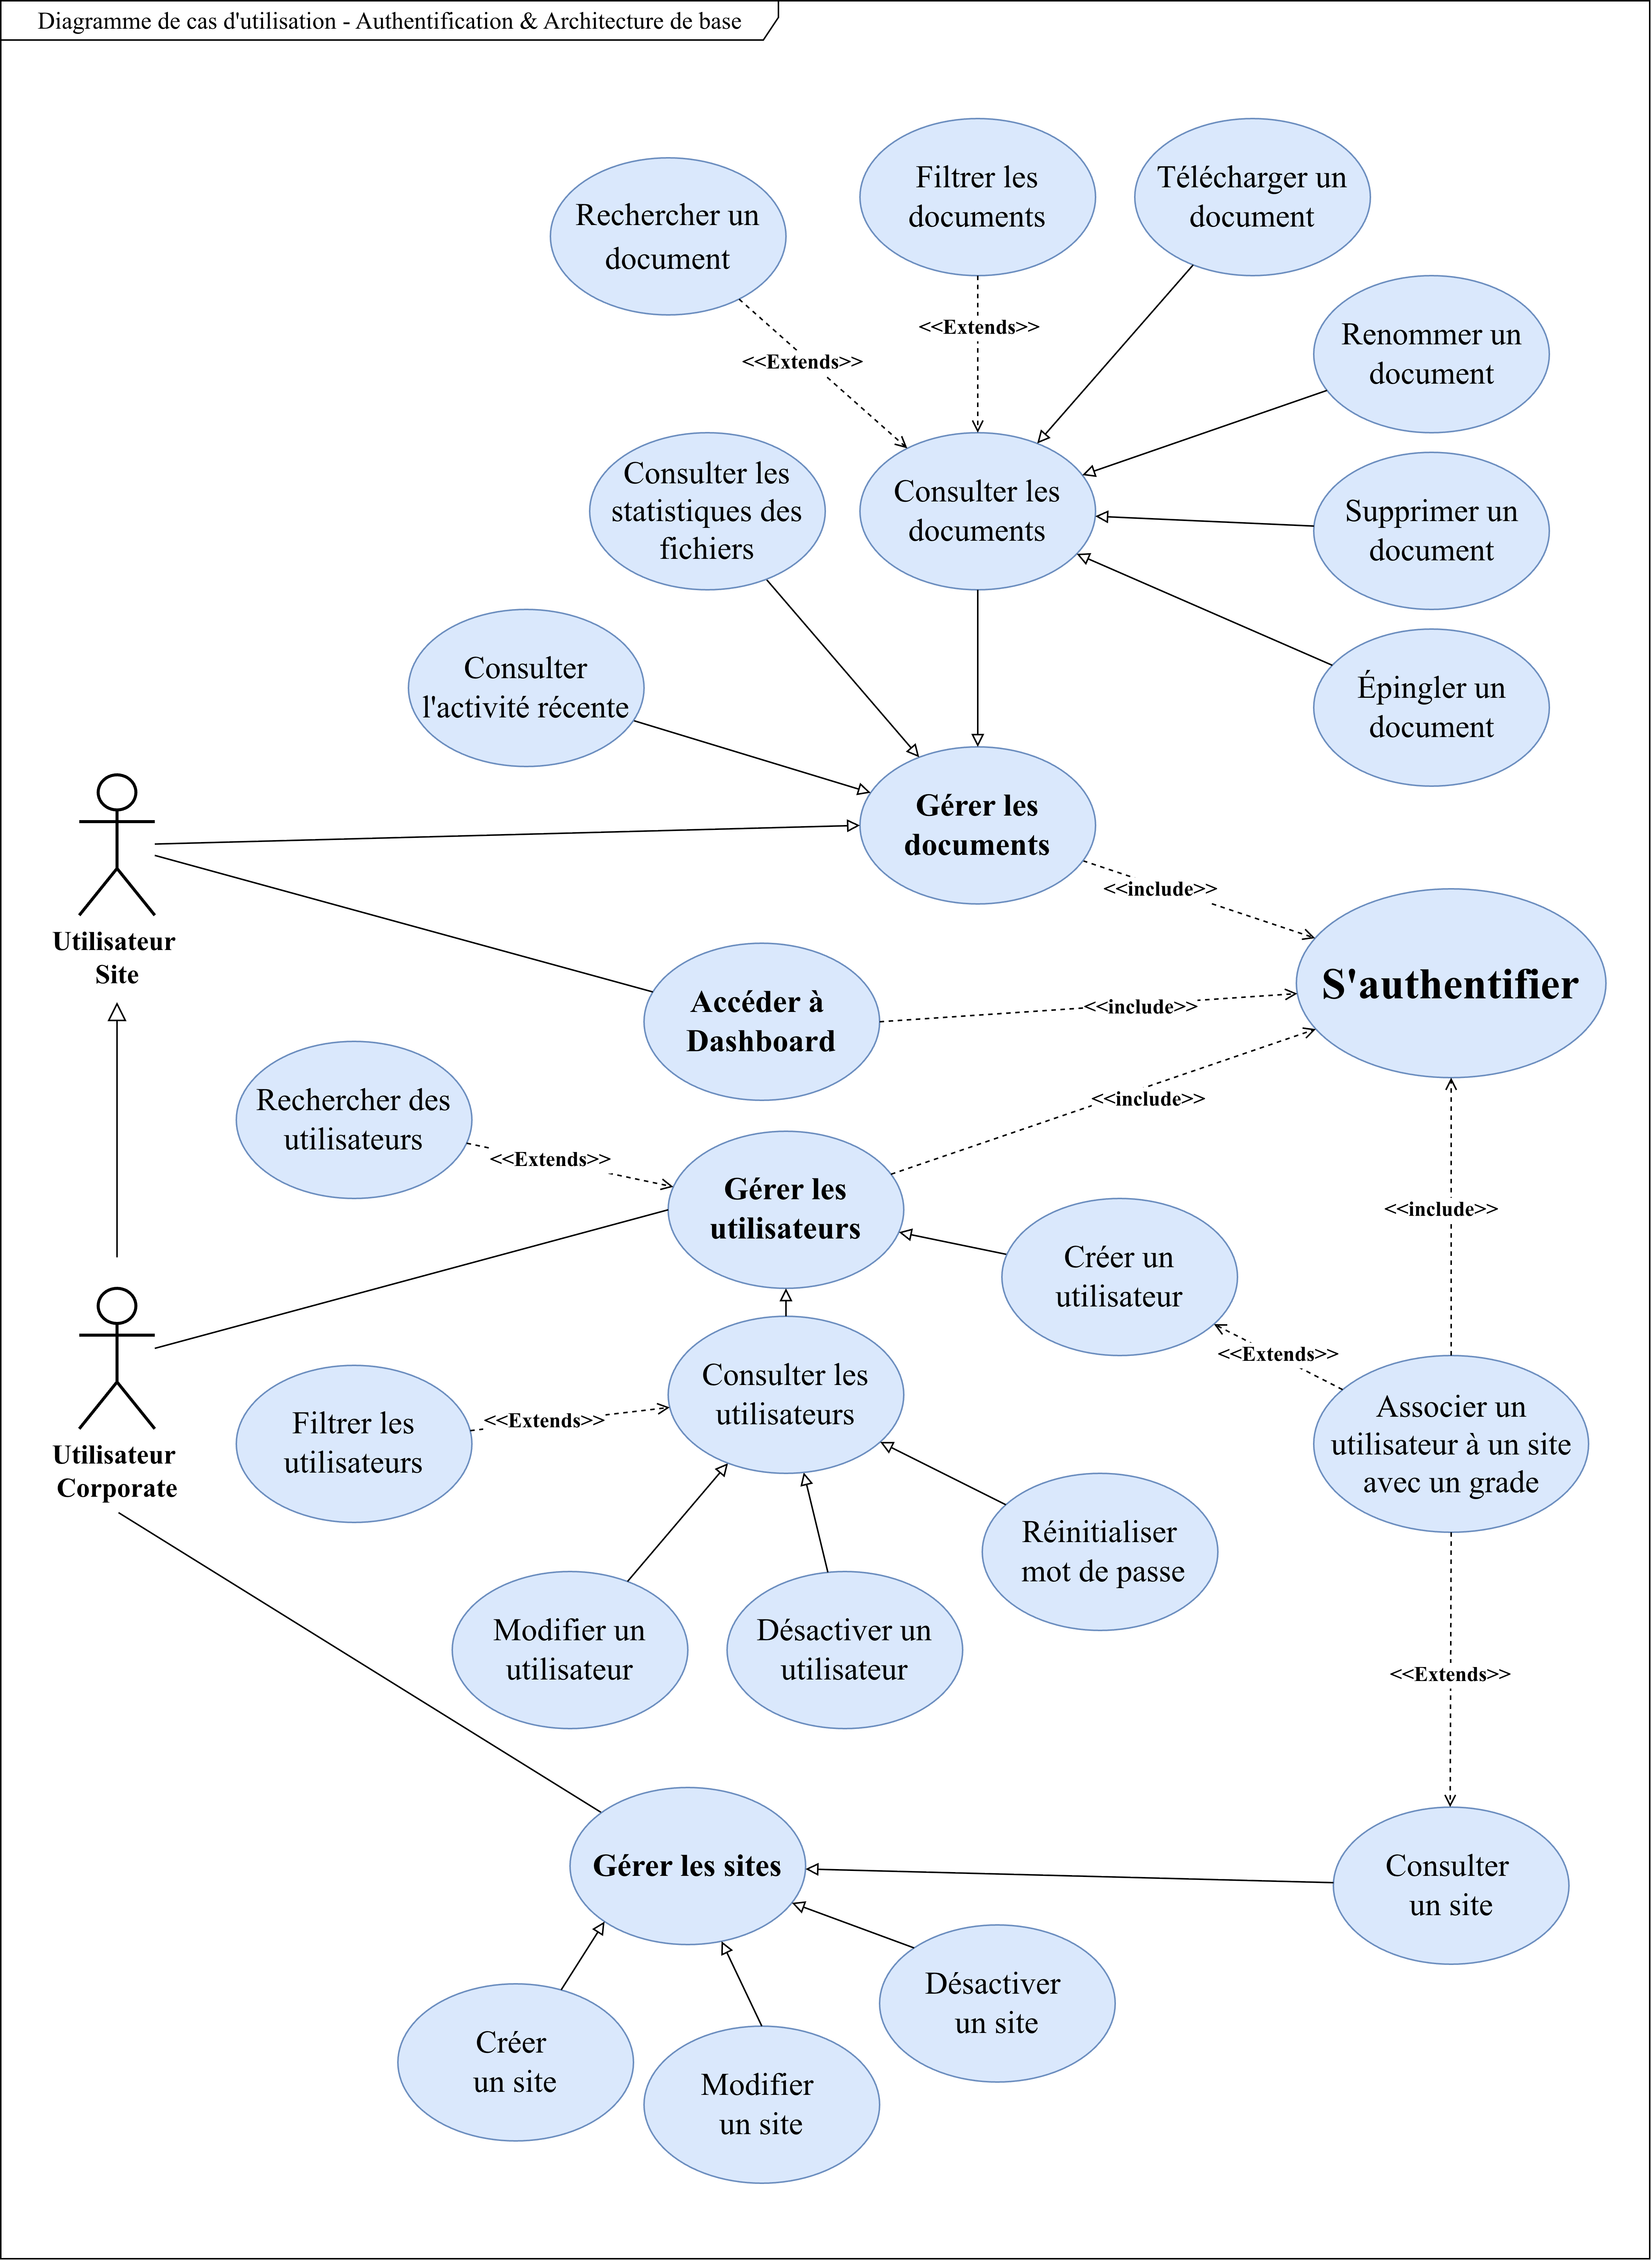
\includegraphics[width=0.92\linewidth]{figures/chapitre-03/diagramme-cas-utilisation-auth-sites-utilisateurs.png}
  \caption{Diagramme de cas d’utilisation — Authentification \& Architecture de base.}
  \label{fig:doc-ch3-1}
\end{figure}

\subsection{Description textuelle du cas d’utilisation : «~Créer un site~»}

Le tableau~\ref{tab:cu-gerer-sites} expose la description textuelle du cas d’utilisation «~Créer un site~».

\begin{table}[H]
  \centering
  \small
  \caption{Description textuelle du cas d’utilisation : «~Créer un site~»}
  \label{tab:cu-gerer-sites}
  \PFETableSetup
  \PFETableRowColors
  \PFETableArrayStretch
  \PFETableTabularXBegin

  \begin{tabularx}{\PFETableBlockWidth}{@{}>{\raggedright\arraybackslash}p{3.2cm} >{\raggedright\arraybackslash}X@{}}
    
    \tableHeaderStyle 
    \tableHeaderCell{Champ} & \tableHeaderCell{Contenu} \\

    \textbf{Titre} & Créer un site \\

    \textbf{Acteurs} & Utilisateur Corporate \\

    \textbf{Objectif} &
    Permettre à l’utilisateur Corporate de créer les sites de Coficab afin d’organiser les activités CSR et structurer l’accès aux données par site. \\

    \textbf{Préconditions} &
    1. L’utilisateur Corporate est authentifié.\par
    2. Un token est obtenu pour accéder aux ressources protégées. \\

    \textbf{Postconditions} &
    1. Les informations du site sont enregistrées.\par
    2. Le nouveau site est disponible pour les autres modules de la plateforme. \\

    \textbf{Scénario nominal} &
    1. L’utilisateur Corporate accède au module de gestion des sites. \par
    2. Le système affiche la liste des sites existants. \par
    3. L’utilisateur choisit l’action : créer un site. \par
    4. L’utilisateur saisit les informations du site (nom, code, pays, région…). \par
    5. Le système valide les données saisies. \par
    6. Si les données sont valides, le système enregistre la création du site et met à jour la liste des sites. \\

    \textbf{Scénario alternatif} &
    \textbf{A. Site déjà existant :} \par
    A.1 L’utilisateur tente de créer un site avec un code déjà existant. \par
    A.2 Le système rejette l’opération. \par
    A.3 Un message est affiché : «~Code site déjà existant~». \\

  \end{tabularx}%

  \PFETableTabularXEnd
\end{table}


\subsection{Description textuelle du cas d’utilisation : «~Créer un utilisateur~»}

Le tableau~\ref{tab:cu-gerer-utilisateurs} expose la description textuelle du cas d’utilisation «~Créer un utilisateur~».

\begin{table}[H]
  \centering
  \small
\caption{Description textuelle du cas d’utilisation : «~Créer un utilisateur~»}
  \label{tab:cu-gerer-utilisateurs}
  \PFETableSetup
  \PFETableRowColors
  \PFETableArrayStretch
  \PFETableTabularXBegin
  \begin{tabularx}{\PFETableBlockWidth}{@{}>{\raggedright\arraybackslash}p{3.2cm} >{\raggedright\arraybackslash}X@{}}
    \tableHeaderStyle \tableHeaderCell{Champ} & \tableHeaderCell{Contenu} \\
    \textbf{Titre} & Créer un utilisateur \\
    \textbf{Acteurs} & Utilisateur Corporate \\
    \textbf{Objectif} &
      Permettre à l’utilisateur Corporate de créer des comptes utilisateurs afin de gérer l’accès à la plateforme. \\
    \textbf{Préconditions} &
      1. L’utilisateur Corporate est authentifié.\par
      2. Un token est obtenu pour accéder aux ressources protégées. \\
    \textbf{Postconditions} &
      1. Les informations du nouvel utilisateur sont enregistrées.\par
      2. Le compte utilisateur est disponible dans la liste des utilisateurs. \\
    \textbf{Scénario nominal} &
      1. L’utilisateur Corporate accède au module de gestion des utilisateurs. \par
      2. Le système affiche la liste des utilisateurs existants. \par
      3. L’utilisateur choisit l’action : créer un utilisateur. \par
      4. L’utilisateur saisit les informations du nouvel utilisateur (nom, email, rôle, site associé, mot de passe…). \par
      5. Le système valide les données saisies. \par
      6. Si les données sont valides, le système enregistre la création de l’utilisateur et met à jour la liste des utilisateurs. \\
    \textbf{Scénario alternatif} &
      \textbf{A. Email déjà utilisé :} \par
      A.1 L’utilisateur Corporate saisit une adresse email déjà existante. \par
      A.2 Le système rejette l’opération. \par
      A.3 Un message est affiché : «~Un utilisateur avec cet email existe déjà~». \par
      \textbf{B. Mot de passe non sécurisé :} \par
      B.1 L’utilisateur Corporate saisit un mot de passe ne respectant pas les critères. \par
      B.2 Le système rejette l’opération. \par
      B.3 Un message est affiché : «~Le mot de passe doit contenir au moins 8 caractères, une majuscule, une minuscule et un caractère spécial~». \\
  \end{tabularx}%
  \PFETableTabularXEnd
\end{table}

\section{Modélisation conceptuelle}

Nous abordons maintenant l'exposé de la conception retenue pour ce premier sprint. À cet effet, nous présentons un diagramme de classe, suivi de la description de plusieurs cas d’utilisation via l'élaboration des diagrammes de séquence appropriés.

\subsection{Diagramme de classe}

Dans le langage UML, le diagramme de classes est un outil essentiel. Il donne une vue claire sur la structure d'un système en décrivant ses classes, leurs attributs, leurs méthodes ainsi que les relations qui les relient entre elles.

La figure~\ref{fig:doc-ch3-2} représente le diagramme de classe du premier sprint.

\begin{figure}[H]
  \centering
  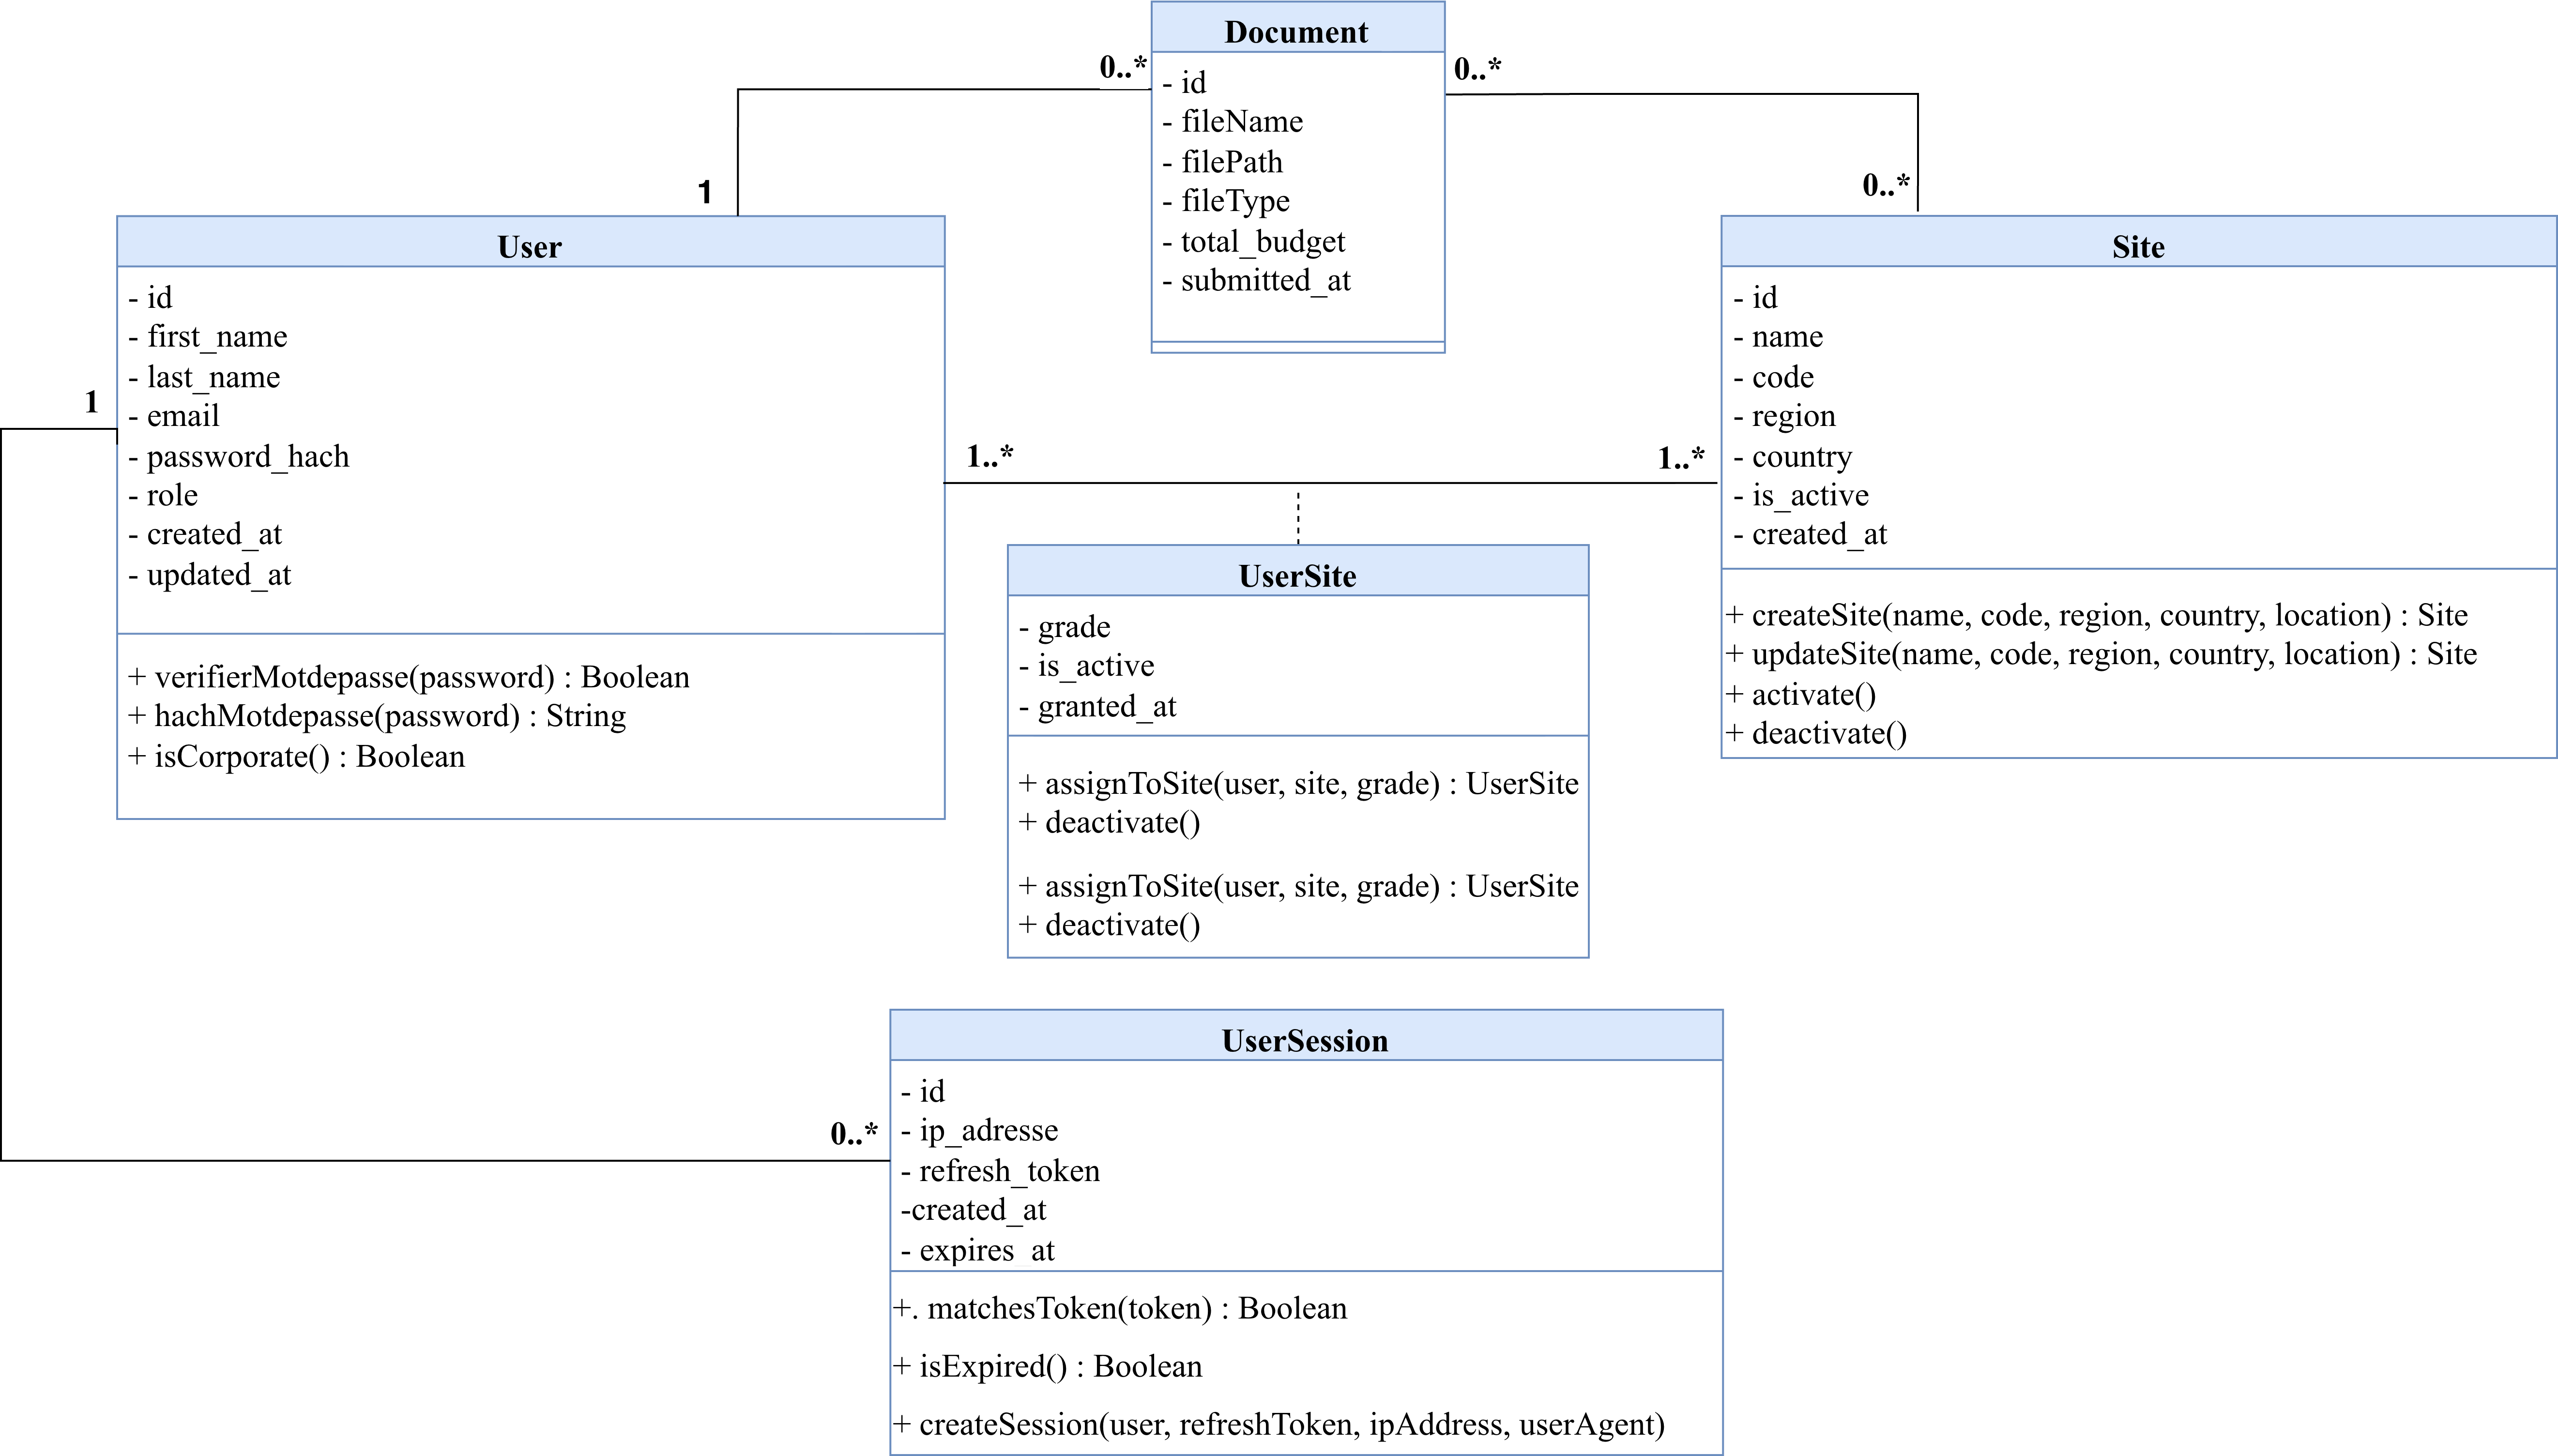
\includegraphics[width=1\linewidth]{figures/chapitre-03/diagramme-classe-auth-sites-documents.png}
  \caption{Diagramme de classe — Authentification \& Architecture de base}
  \label{fig:doc-ch3-2}
\end{figure}

\subsection{Diagramme de séquence}

Les diagrammes de séquences montrent les échanges entre les objets du système. Nous avons documenté les principaux cas d’utilisation du premier sprint : «~S’authentifier~», «~Créer un site~» et «~Créer un utilisateur~».

\subsubsection{Diagramme de séquence : «~S’authentifier~»}

La figure~\ref{fig:doc-ch3-seq-auth} présente le diagramme de séquence du cas d’utilisation «~S’authentifier~».

\IfFileExists{figures/chapitre-03/diagramme-sequence-s-authentifier.png}{%
\begin{figure}[H]
  \centering
  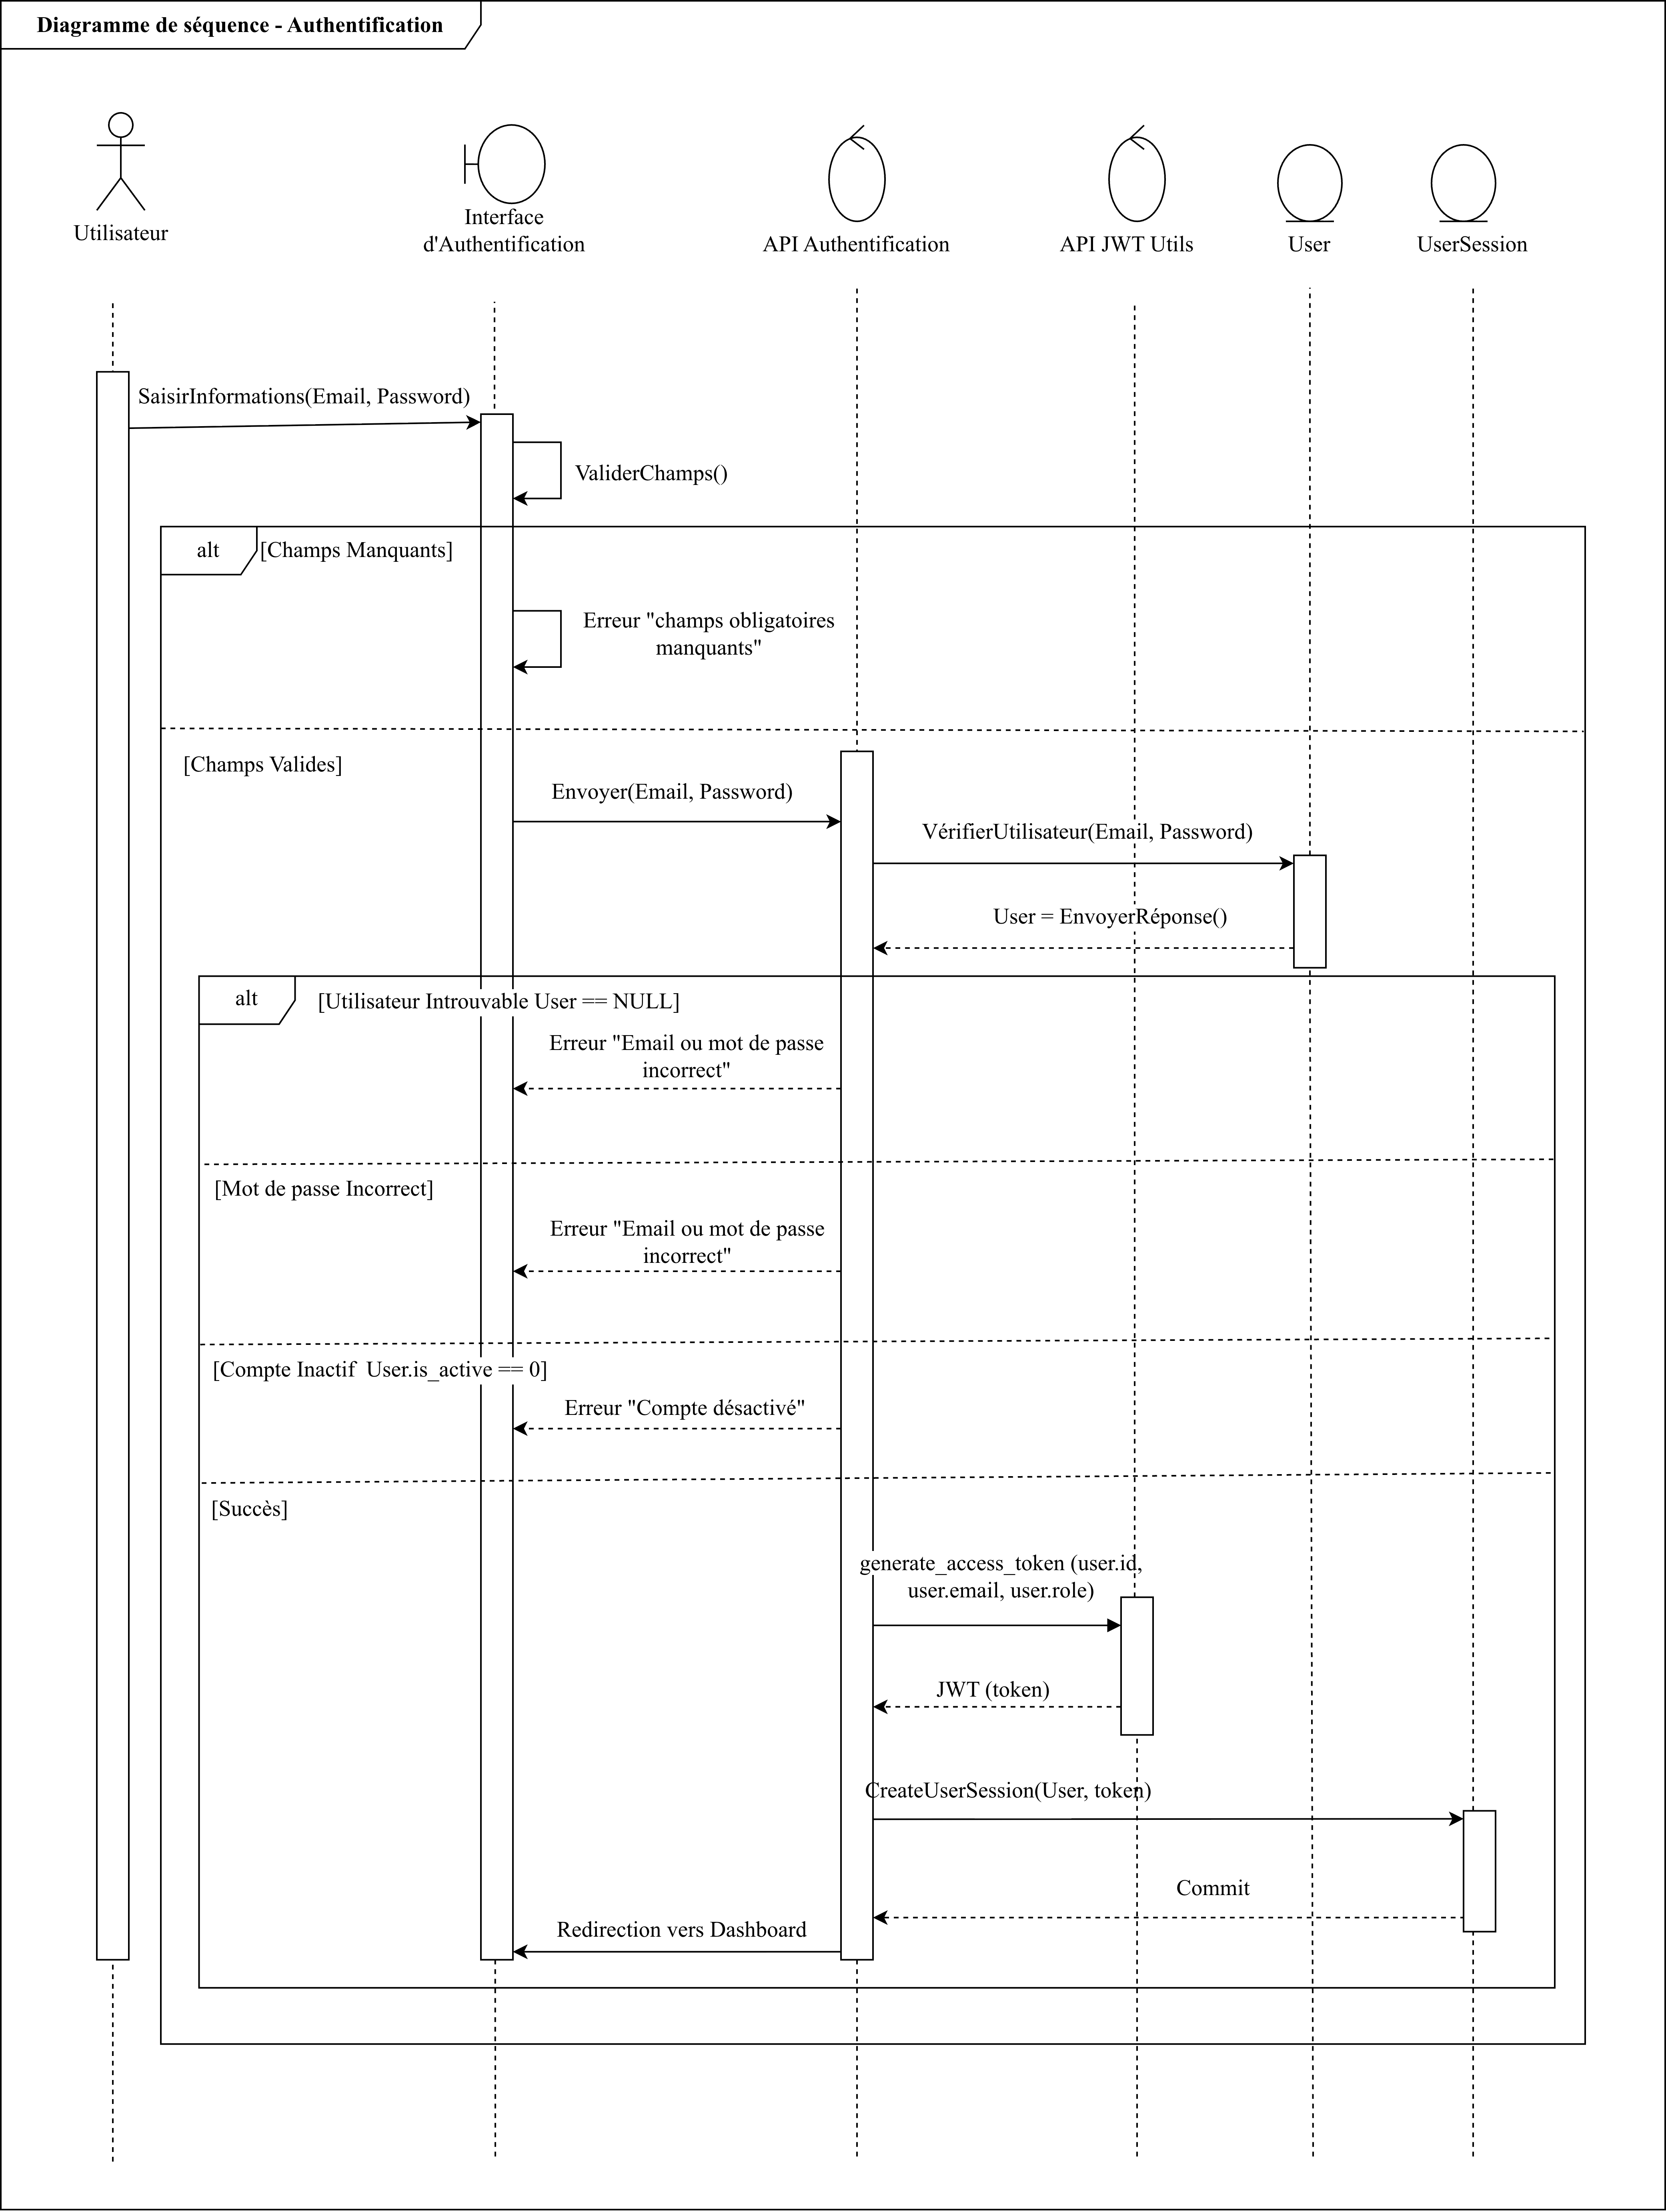
\includegraphics[width=0.92\linewidth]{figures/chapitre-03/diagramme-sequence-s-authentifier.png}
  \caption{Diagramme de séquence — «~S’authentifier~».}
  \label{fig:doc-ch3-seq-auth}
\end{figure}%
}{%
\begin{figure}[H]
  \centering
  \fbox{\parbox{0.92\linewidth}{\centering\vspace{3.2cm}\textit{(Figure à insérer : \texttt{figures/chapitre-03/diagramme-sequence-s-authentifier.png})}\vspace{3.2cm}}}
  \caption{Diagramme de séquence — «~S’authentifier~».}
  \label{fig:doc-ch3-seq-auth}
\end{figure}%
}

\subsubsection{Diagramme de séquence : «~Créer un site~»}

La figure~\ref{fig:doc-ch3-seq-site} présente le diagramme de séquence du cas d’utilisation «~Créer un site~».

\IfFileExists{figures/chapitre-03/diagramme-sequence-creer-un-site.png}{%
\begin{figure}[H]
  \centering
  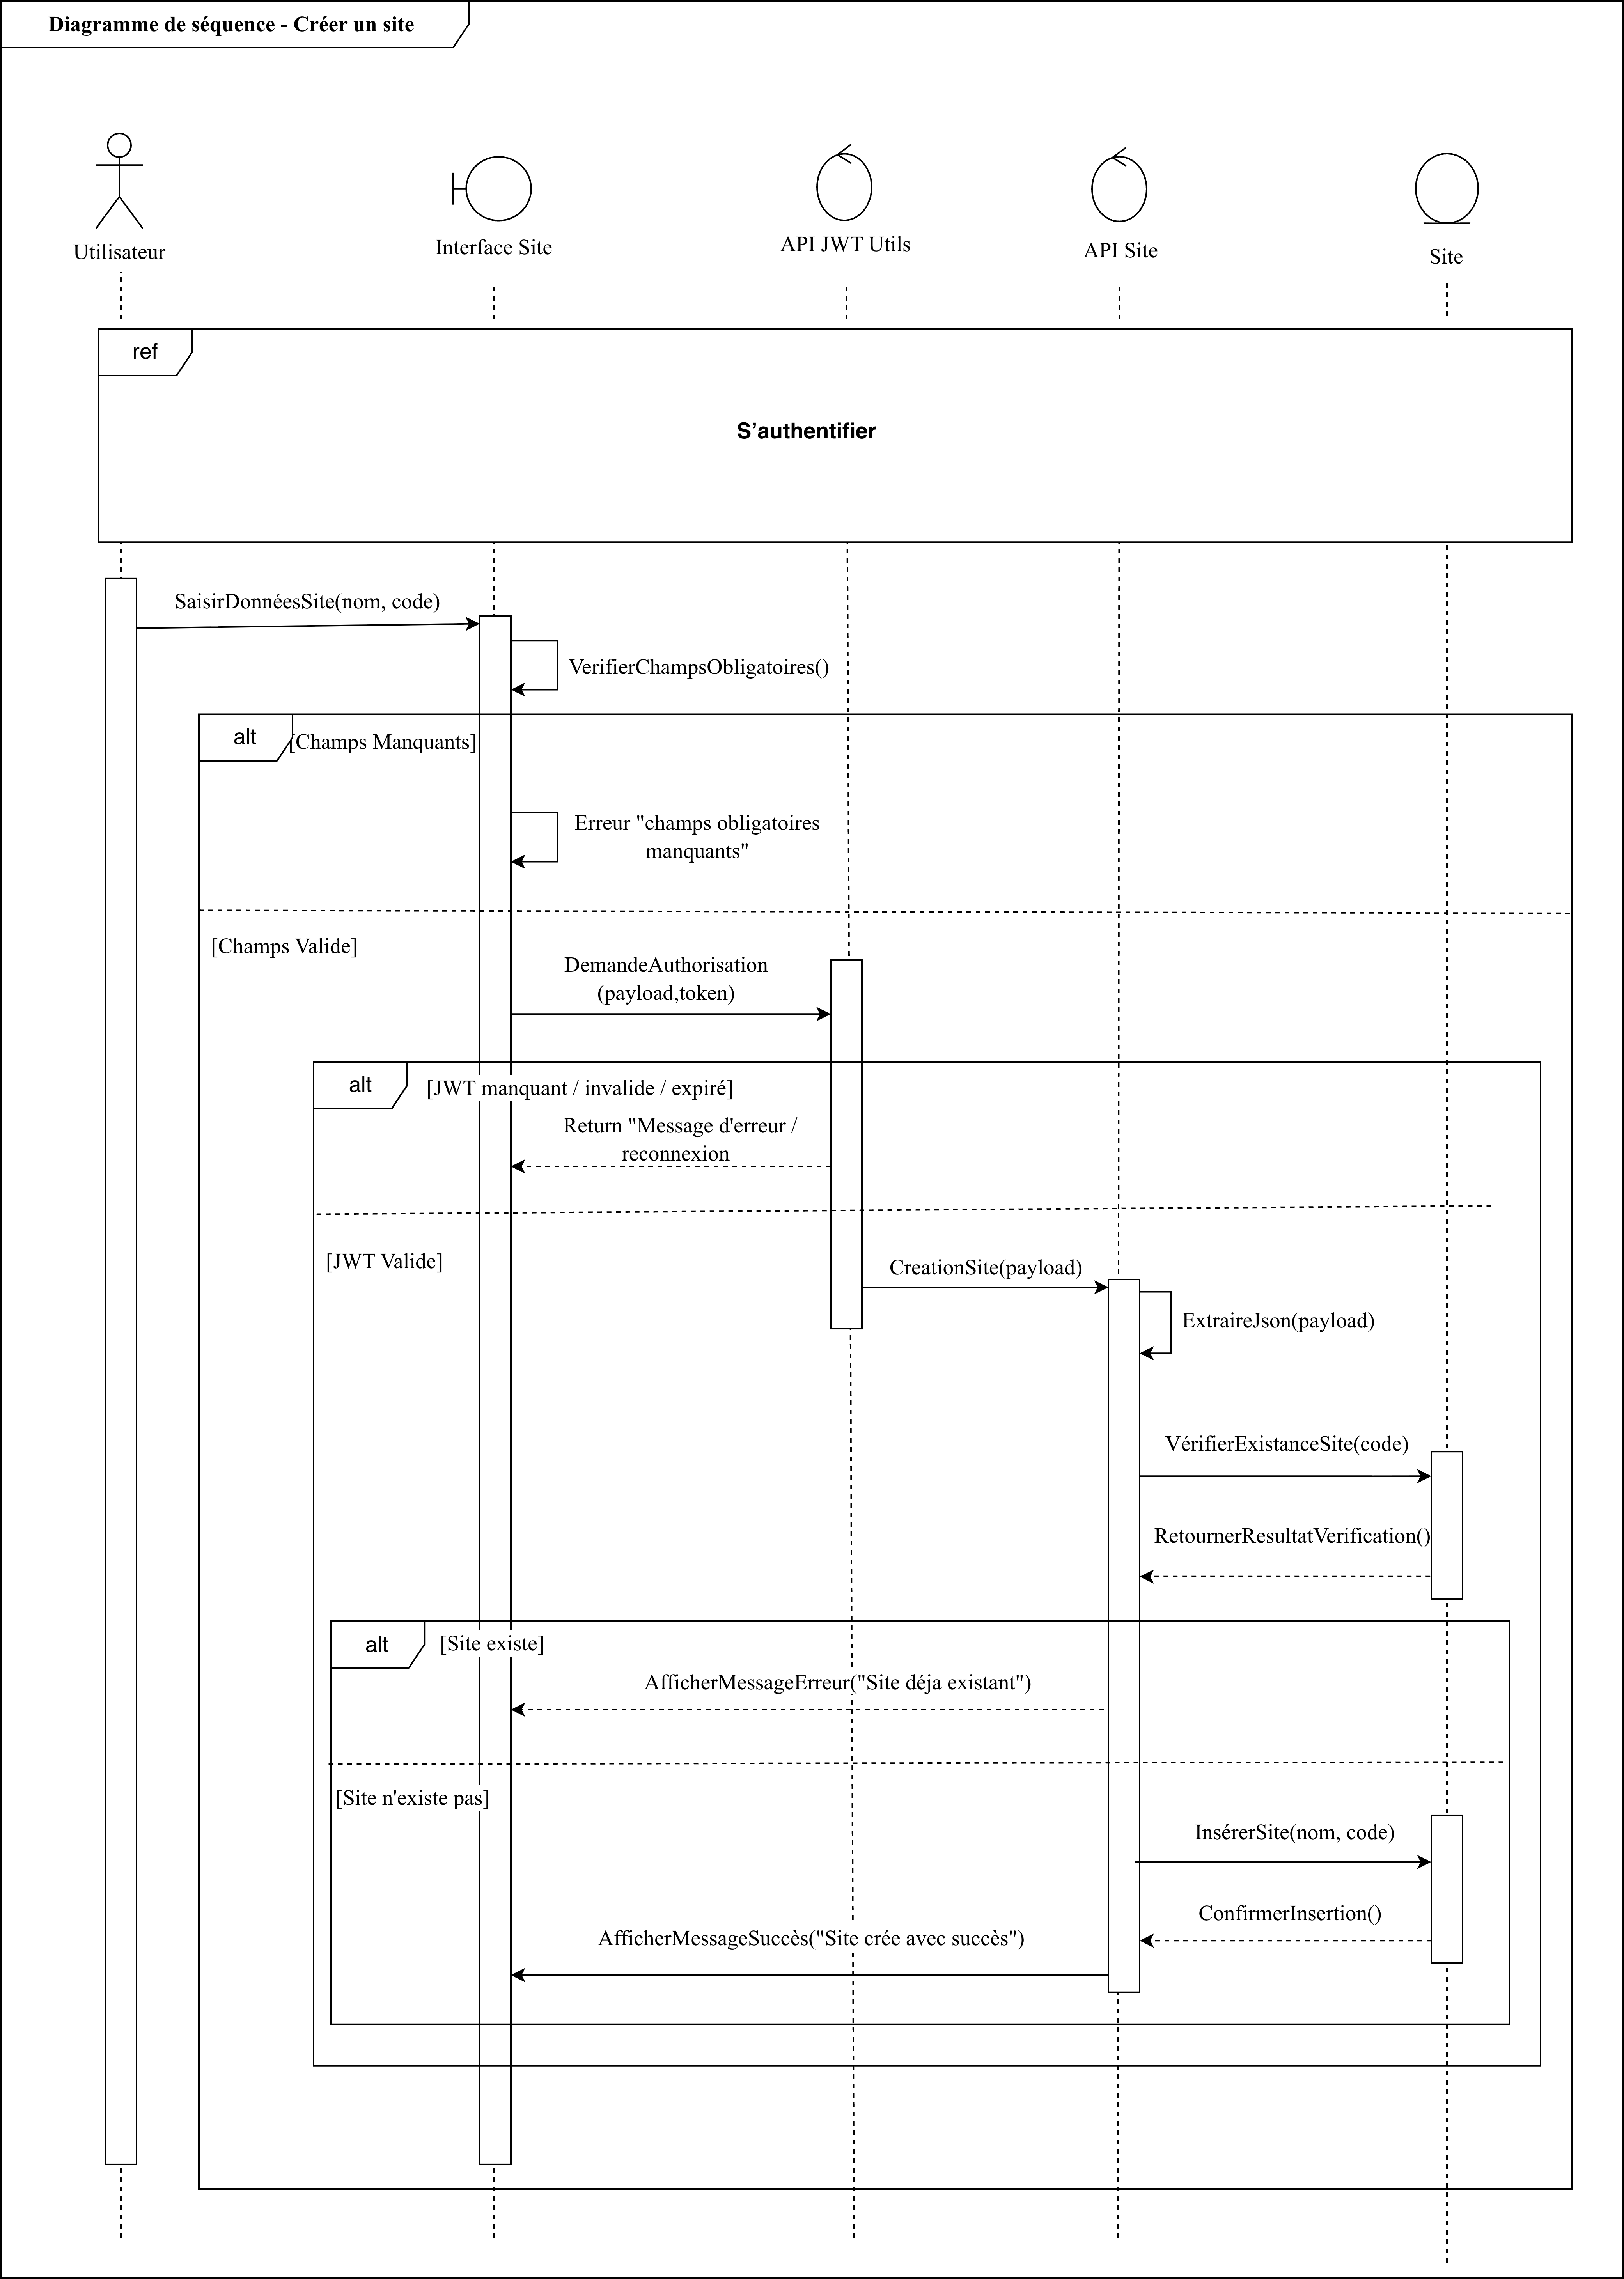
\includegraphics[width=0.92\linewidth]{figures/chapitre-03/diagramme-sequence-creer-un-site.png}
  \caption{Diagramme de séquence — «~Créer un site~».}
  \label{fig:doc-ch3-seq-site}
\end{figure}%
}{%
\begin{figure}[H]
  \centering
  \fbox{\parbox{0.92\linewidth}{\centering\vspace{3.2cm}\textit{(Figure à insérer : \texttt{figures/chapitre-03/diagramme-sequence-creer-un-site.png})}\vspace{3.2cm}}}
  \caption{Diagramme de séquence — «~Créer un site~».}
  \label{fig:doc-ch3-seq-site}
\end{figure}%
}

\subsubsection{Diagramme de séquence : «~Créer un utilisateur~»}

La figure~\ref{fig:doc-ch3-seq-user} présente le diagramme de séquence du cas d’utilisation «~Créer un utilisateur~».

\IfFileExists{figures/chapitre-03/diagramme-sequence-creer-un-utilisateur.png}{%
\begin{figure}[H]
  \centering
  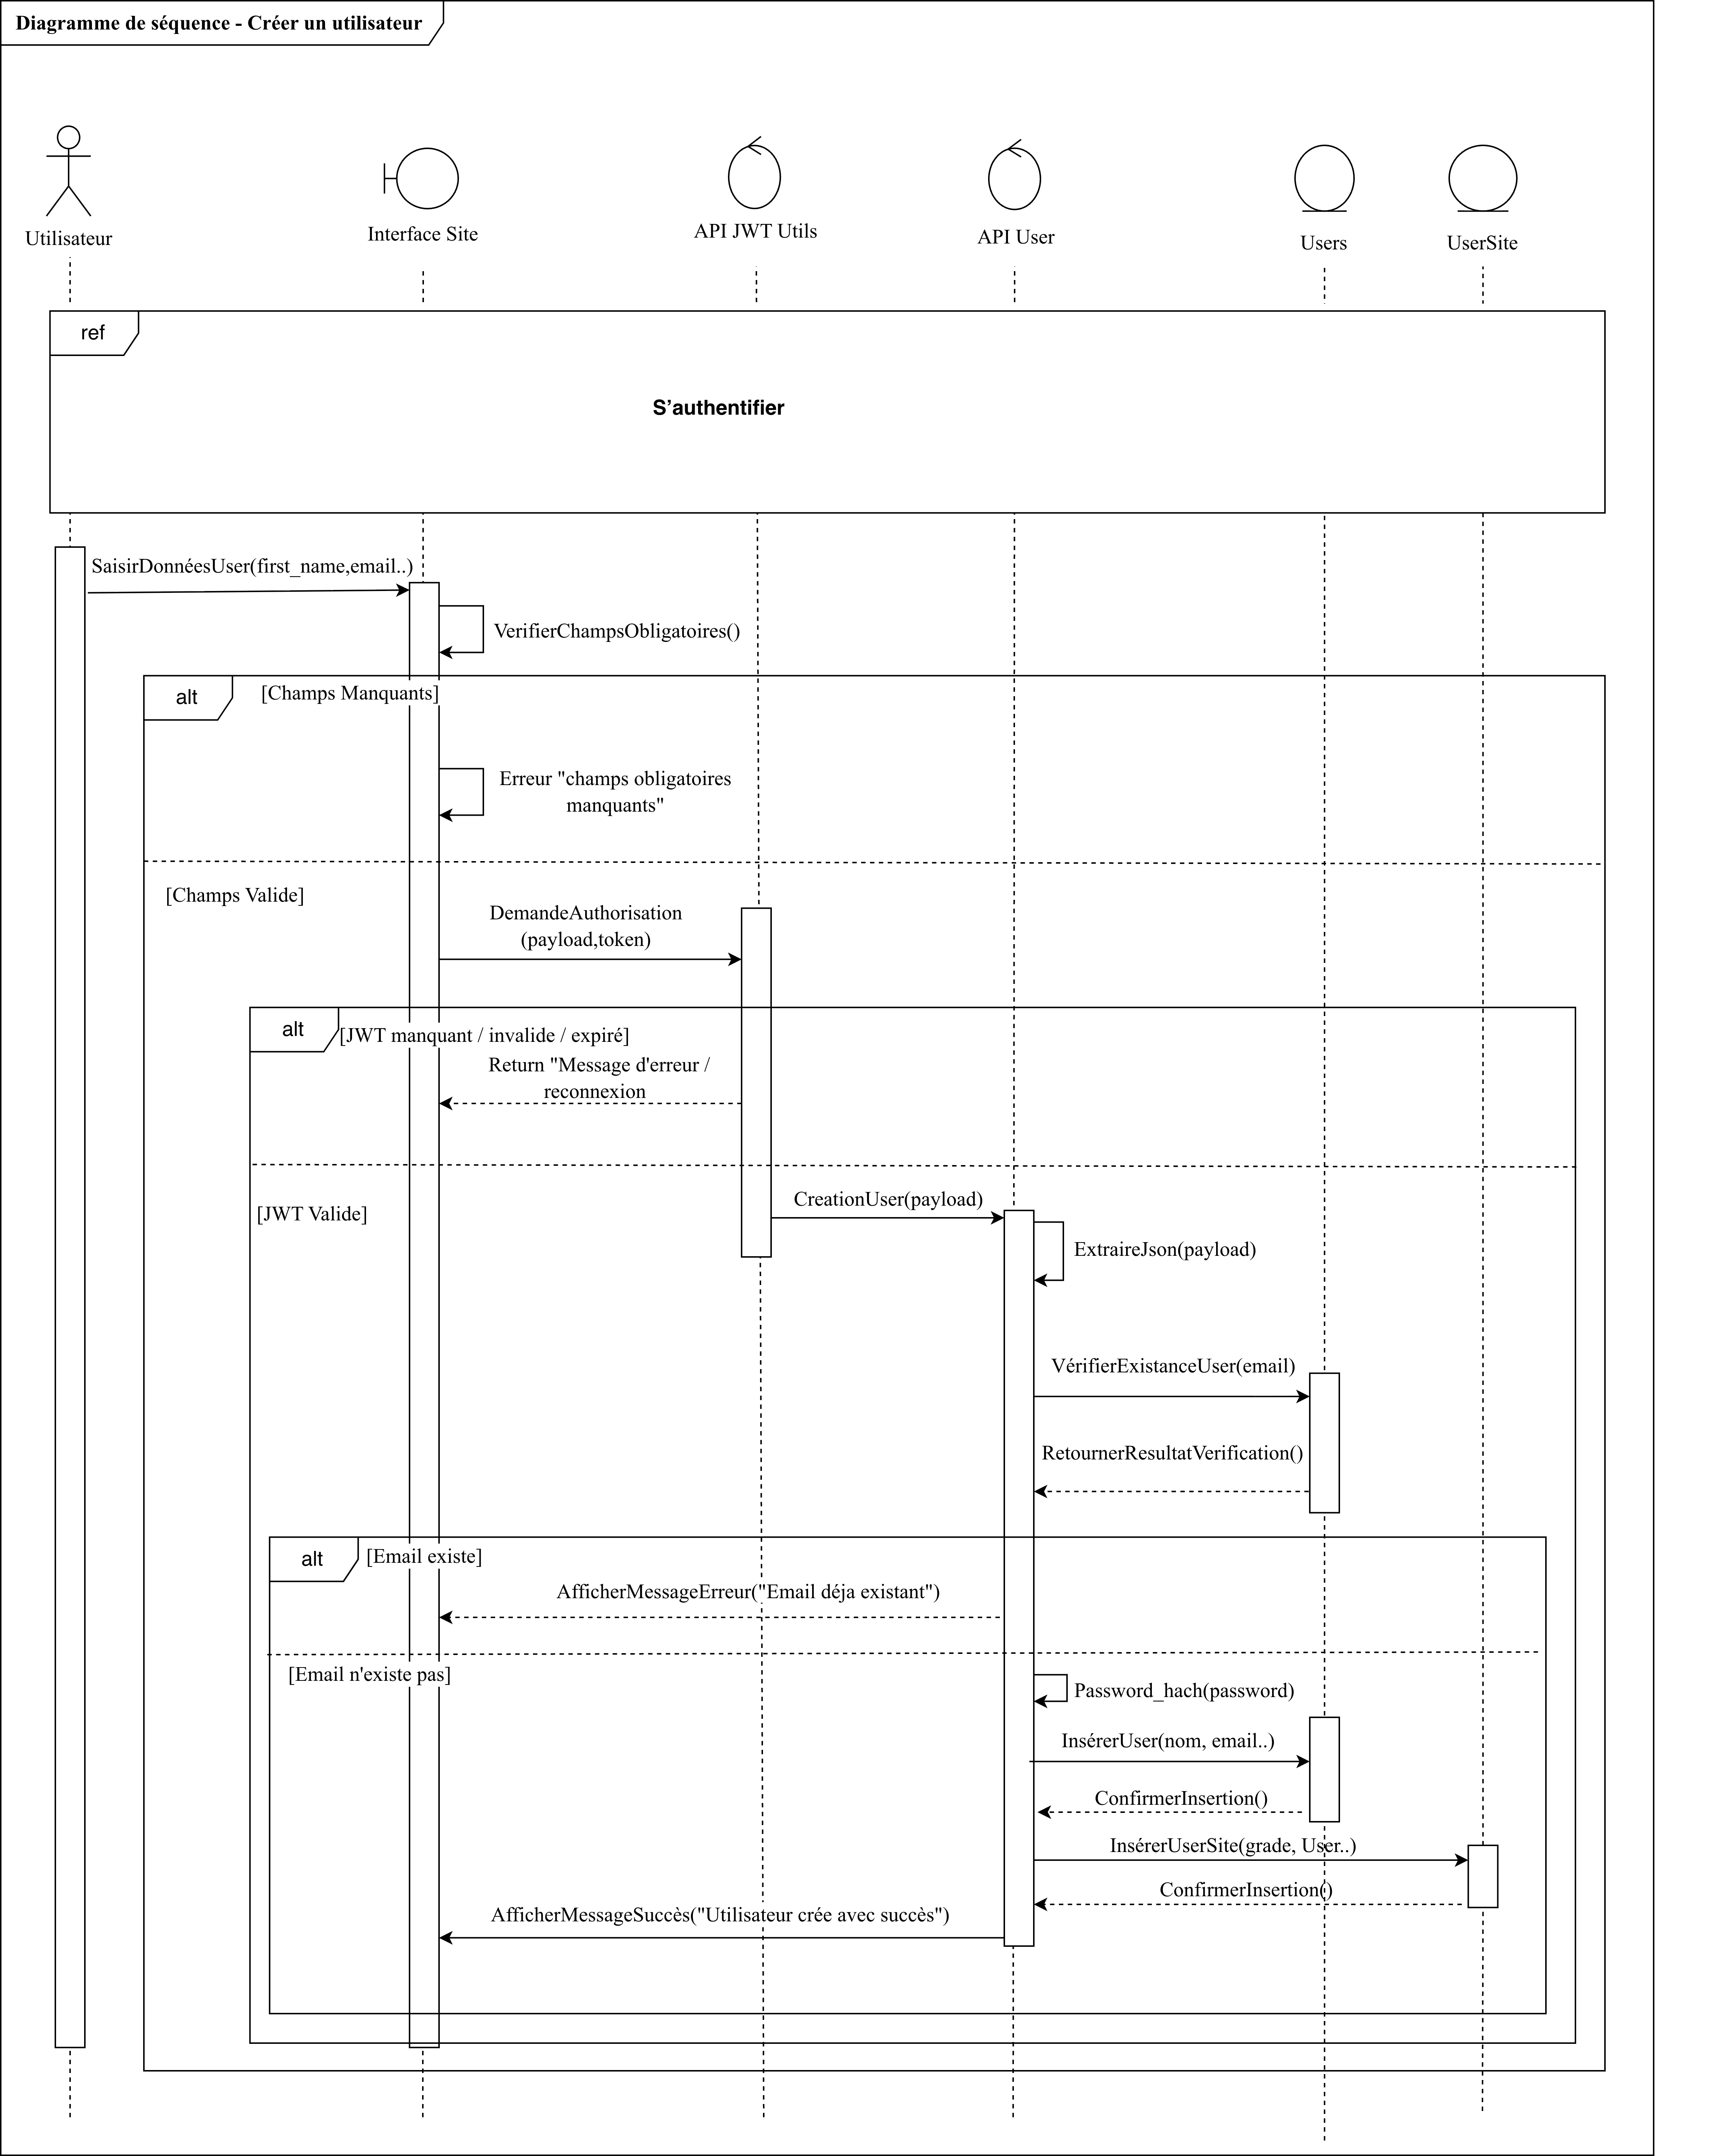
\includegraphics[width=1\linewidth]{figures/chapitre-03/diagramme-sequence-creer-un-utilisateur.png}
  \caption{Diagramme de séquence — «~Créer un utilisateur~».}
  \label{fig:doc-ch3-seq-user}
\end{figure}%
}{%
\begin{figure}[H]
  \centering
  \fbox{\parbox{1\linewidth}{\centering\vspace{3.2cm}\textit{(Figure à insérer : \texttt{figures/chapitre-03/diagramme-sequence-creer-un-utilisateur.png})}\vspace{3.2cm}}}
  \caption{Diagramme de séquence — «~Créer un utilisateur~».}
  \label{fig:doc-ch3-seq-user}
\end{figure}%
}

\subsection{Diagramme d’activité}

Les diagrammes d’activité illustrent le déroulement des traitements métier et les décisions principales pour les cas d'utilisation du sprint 1.

\subsubsection{Diagramme d’activité : «~S’authentifier~»}

La figure~\ref{fig:doc-ch3-act-auth} présente le diagramme d’activité du cas d’utilisation «~S’authentifier~».

\IfFileExists{figures/chapitre-03/Diagramme_dactivite_Sauthentifier.png}{%
\begin{figure}[H]
  \centering
  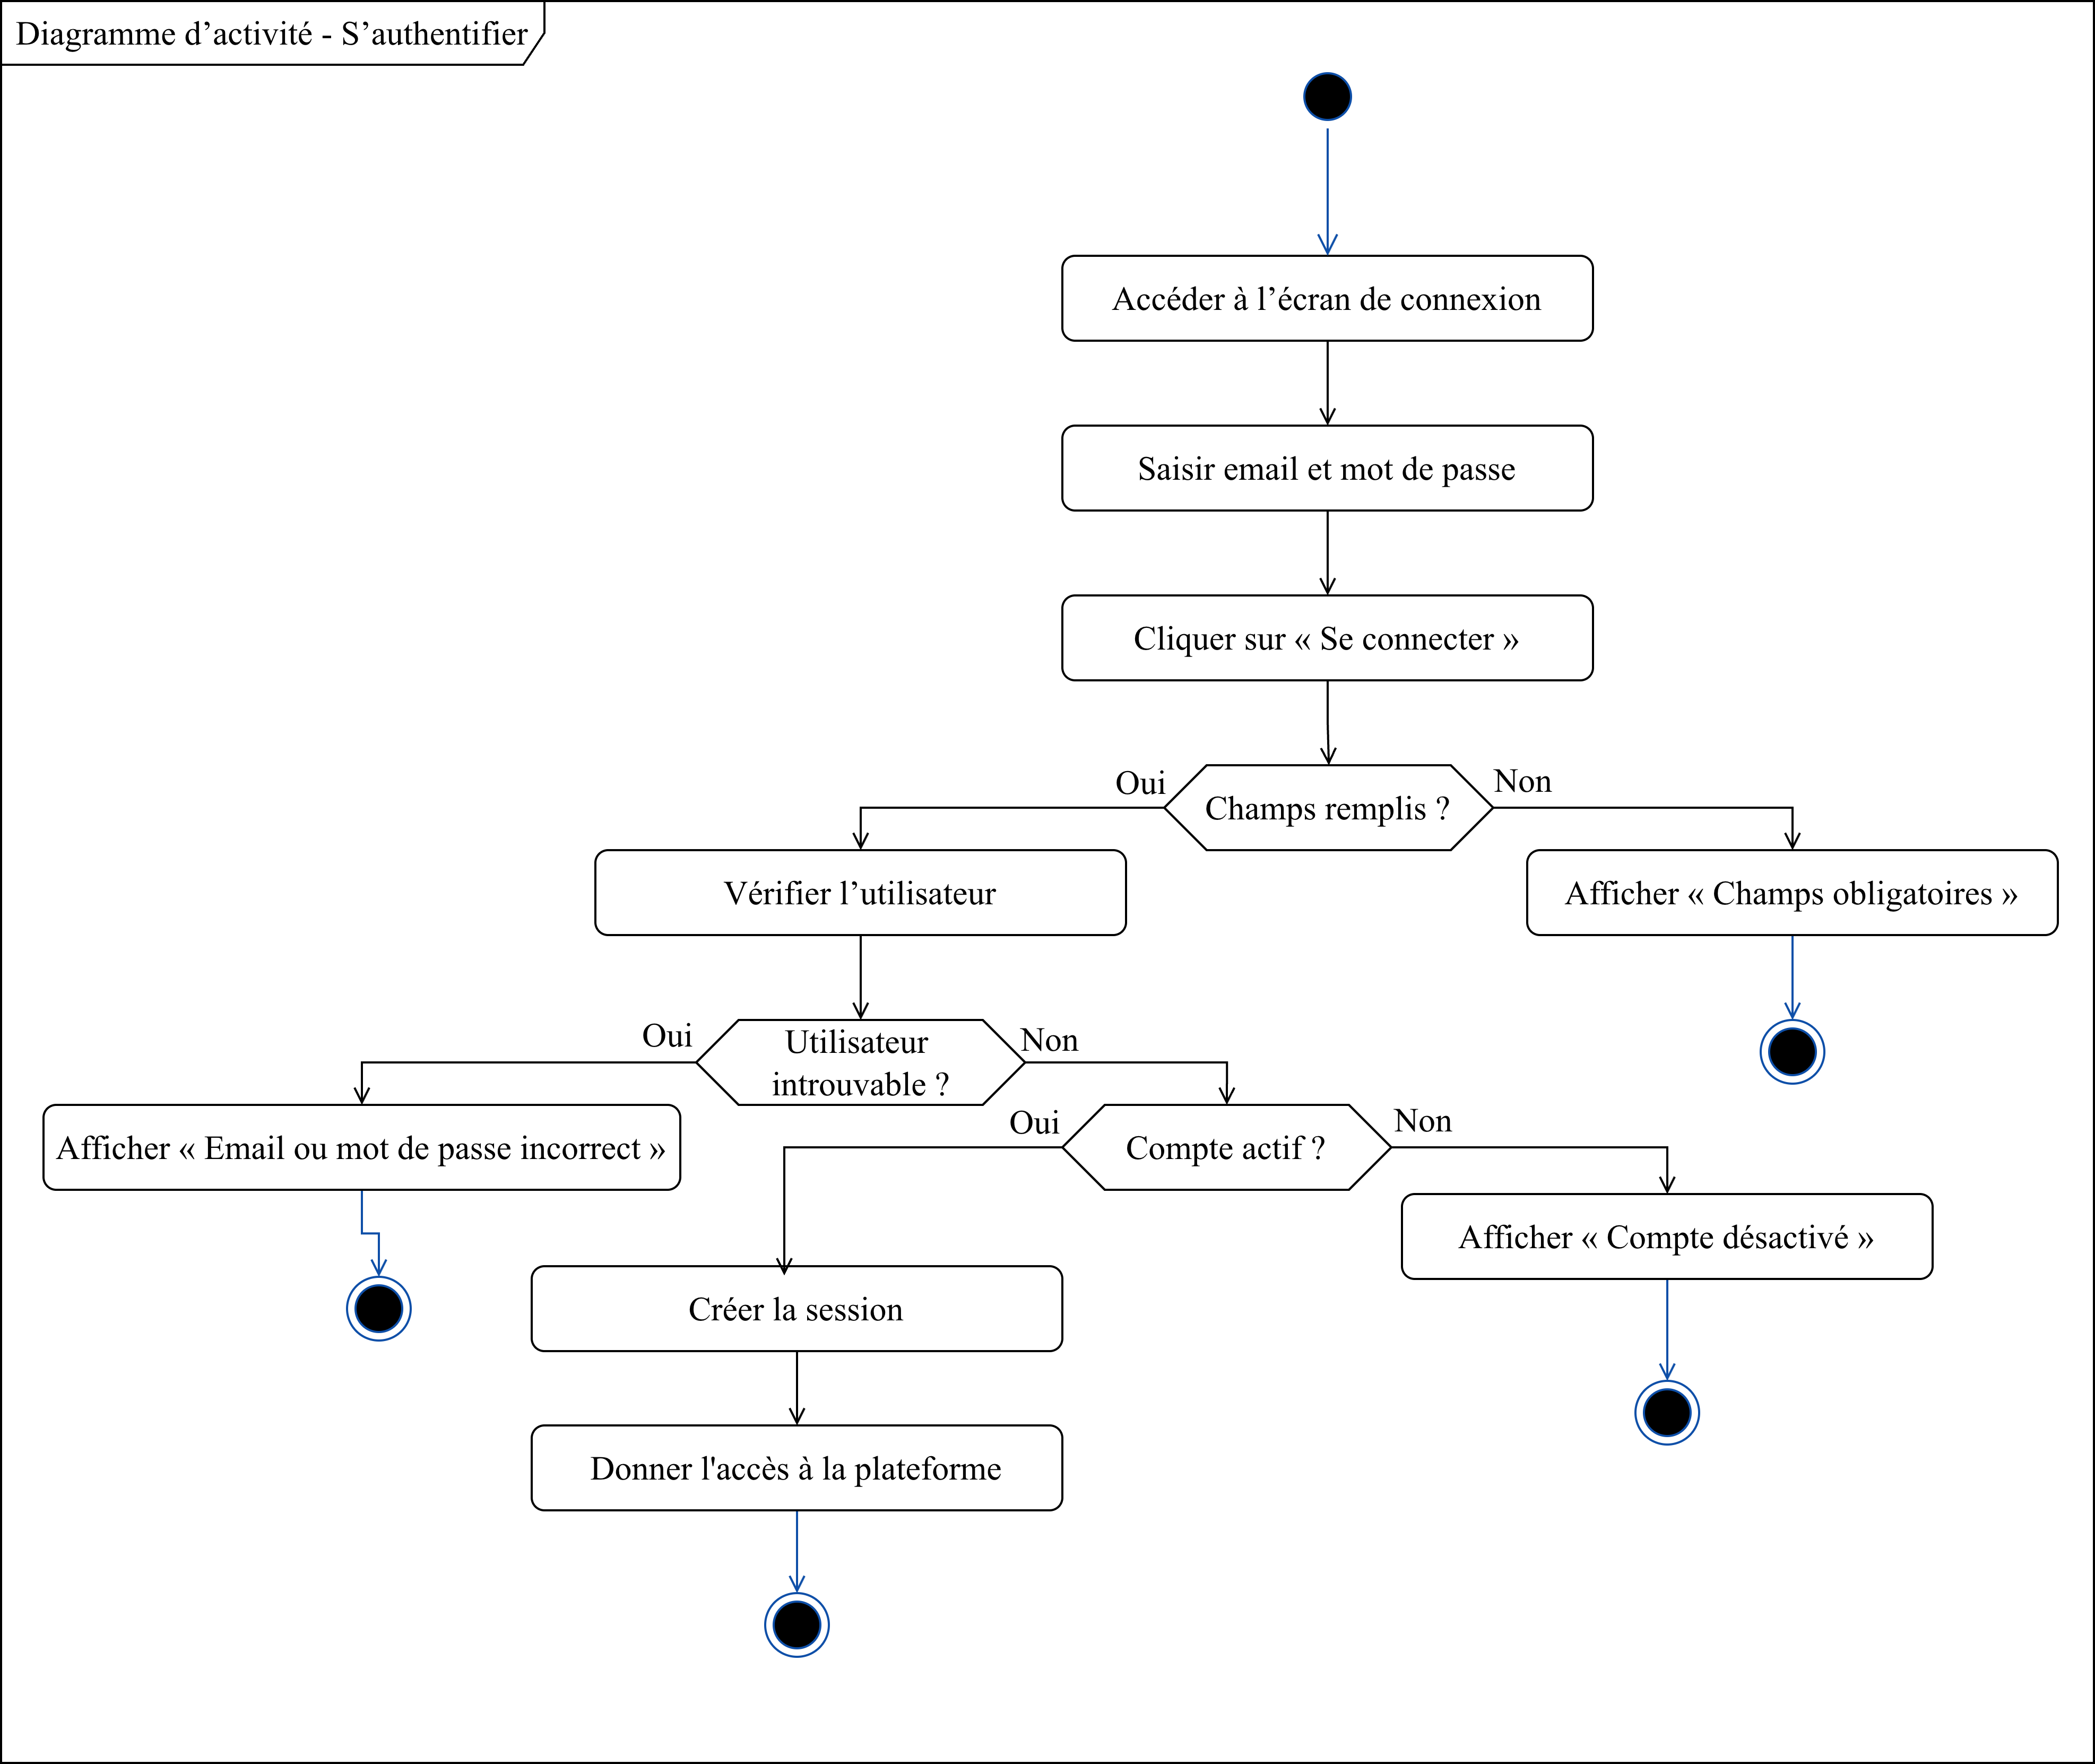
\includegraphics[width=0.92\linewidth]{figures/chapitre-03/Diagramme_dactivite_Sauthentifier.png}
  \caption{Diagramme d’activité — «~S’authentifier~».}
  \label{fig:doc-ch3-act-auth}
\end{figure}%
}{%
\begin{figure}[H]
  \centering
  \fbox{\parbox{0.92\linewidth}{\centering\vspace{3.2cm}\textit{(Figure à insérer : \texttt{figures/chapitre-03/Diagramme\_dactivite\_Sauthentifier.png})}\vspace{3.2cm}}}
  \caption{Diagramme d’activité — «~S’authentifier~».}
  \label{fig:doc-ch3-act-auth}
\end{figure}%
}

\subsubsection{Diagramme d’activité : «~Créer un site~»}

La figure~\ref{fig:doc-ch3-act-site} présente le diagramme d’activité du cas d’utilisation «~Créer un site~».

\IfFileExists{figures/chapitre-03/Diagramme_dactivite_cree_un_site.png}{%
\begin{figure}[H]
  \centering
  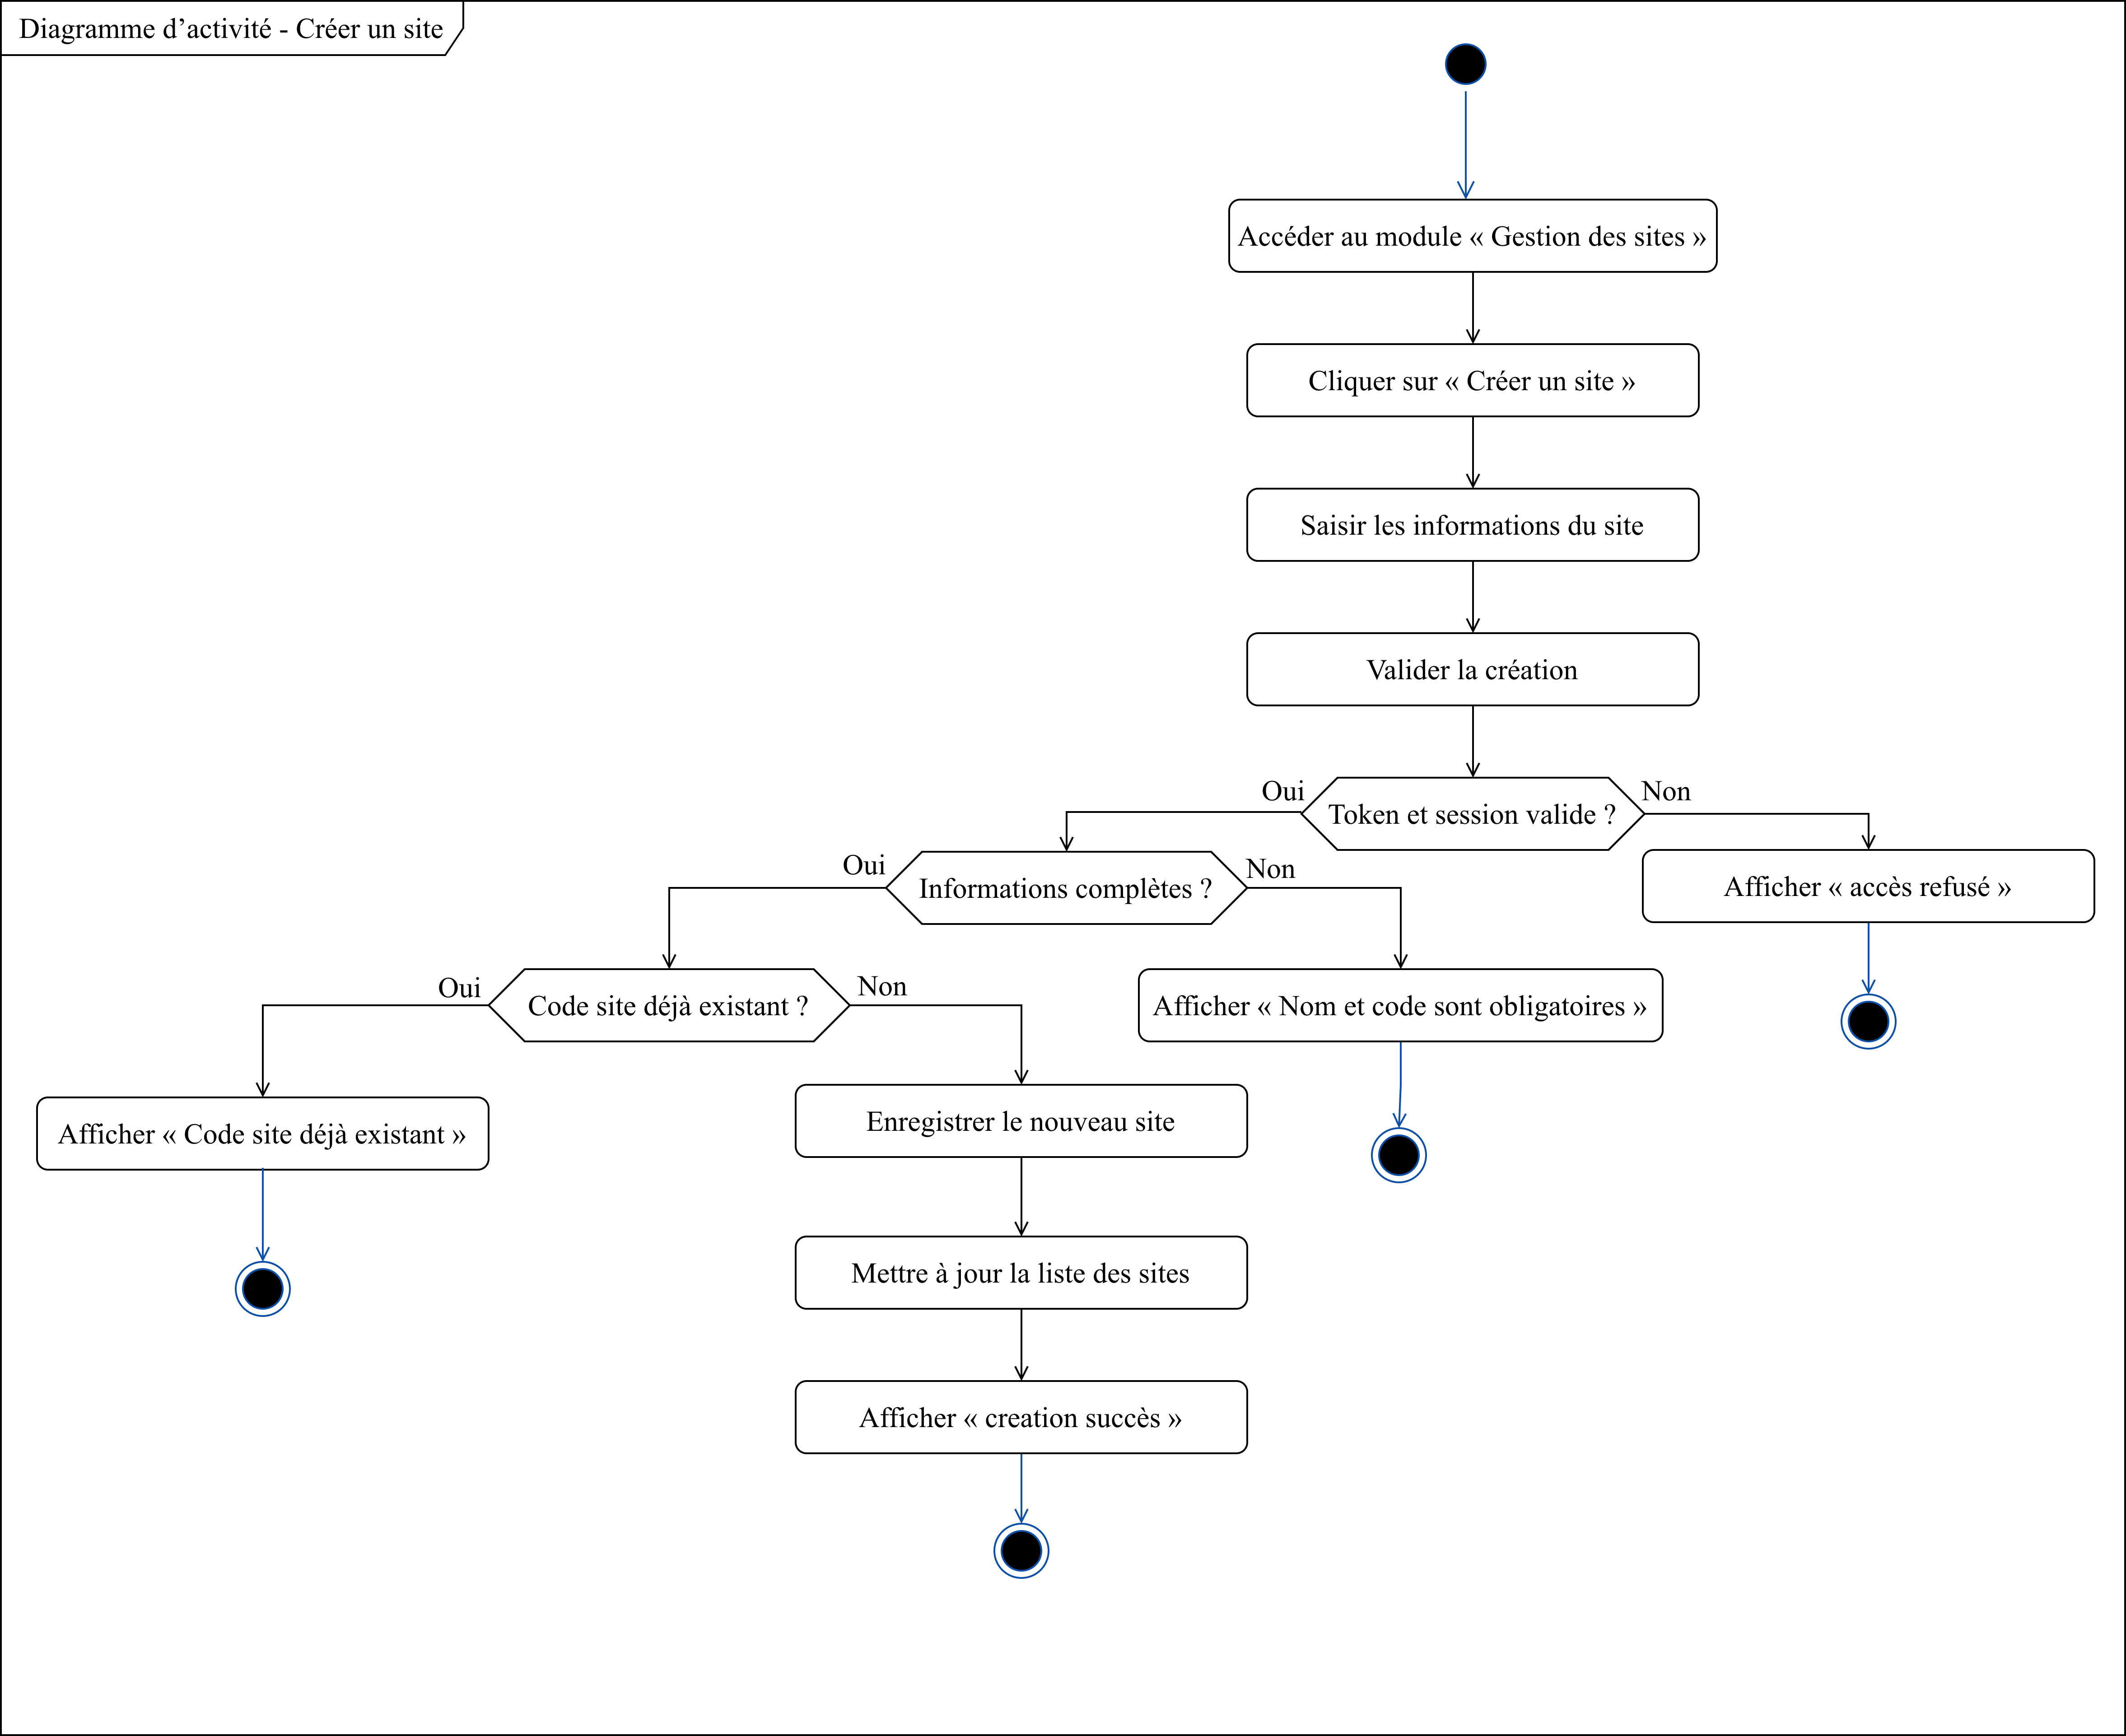
\includegraphics[width=0.92\linewidth]{figures/chapitre-03/Diagramme_dactivite_cree_un_site.png}
  \caption{Diagramme d’activité — «~Créer un site~».}
  \label{fig:doc-ch3-act-site}
\end{figure}%
}{%
\begin{figure}[H]
  \centering
  \fbox{\parbox{0.92\linewidth}{\centering\vspace{3.2cm}\textit{(Figure à insérer : \texttt{figures/chapitre-03/Diagramme\_dactivite\_cree\_un\_site.png})}\vspace{3.2cm}}}
  \caption{Diagramme d’activité — «~Créer un site~».}
  \label{fig:doc-ch3-act-site}
\end{figure}%
}

\subsubsection{Diagramme d’activité : «~Créer un utilisateur~»}

La figure~\ref{fig:doc-ch3-act-user} présente le diagramme d’activité du cas d’utilisation «~Créer un utilisateur~».

\IfFileExists{figures/chapitre-03/Diagramme_dactivite_cree_un_utilisateur.png}{%
\begin{figure}[H]
  \centering
  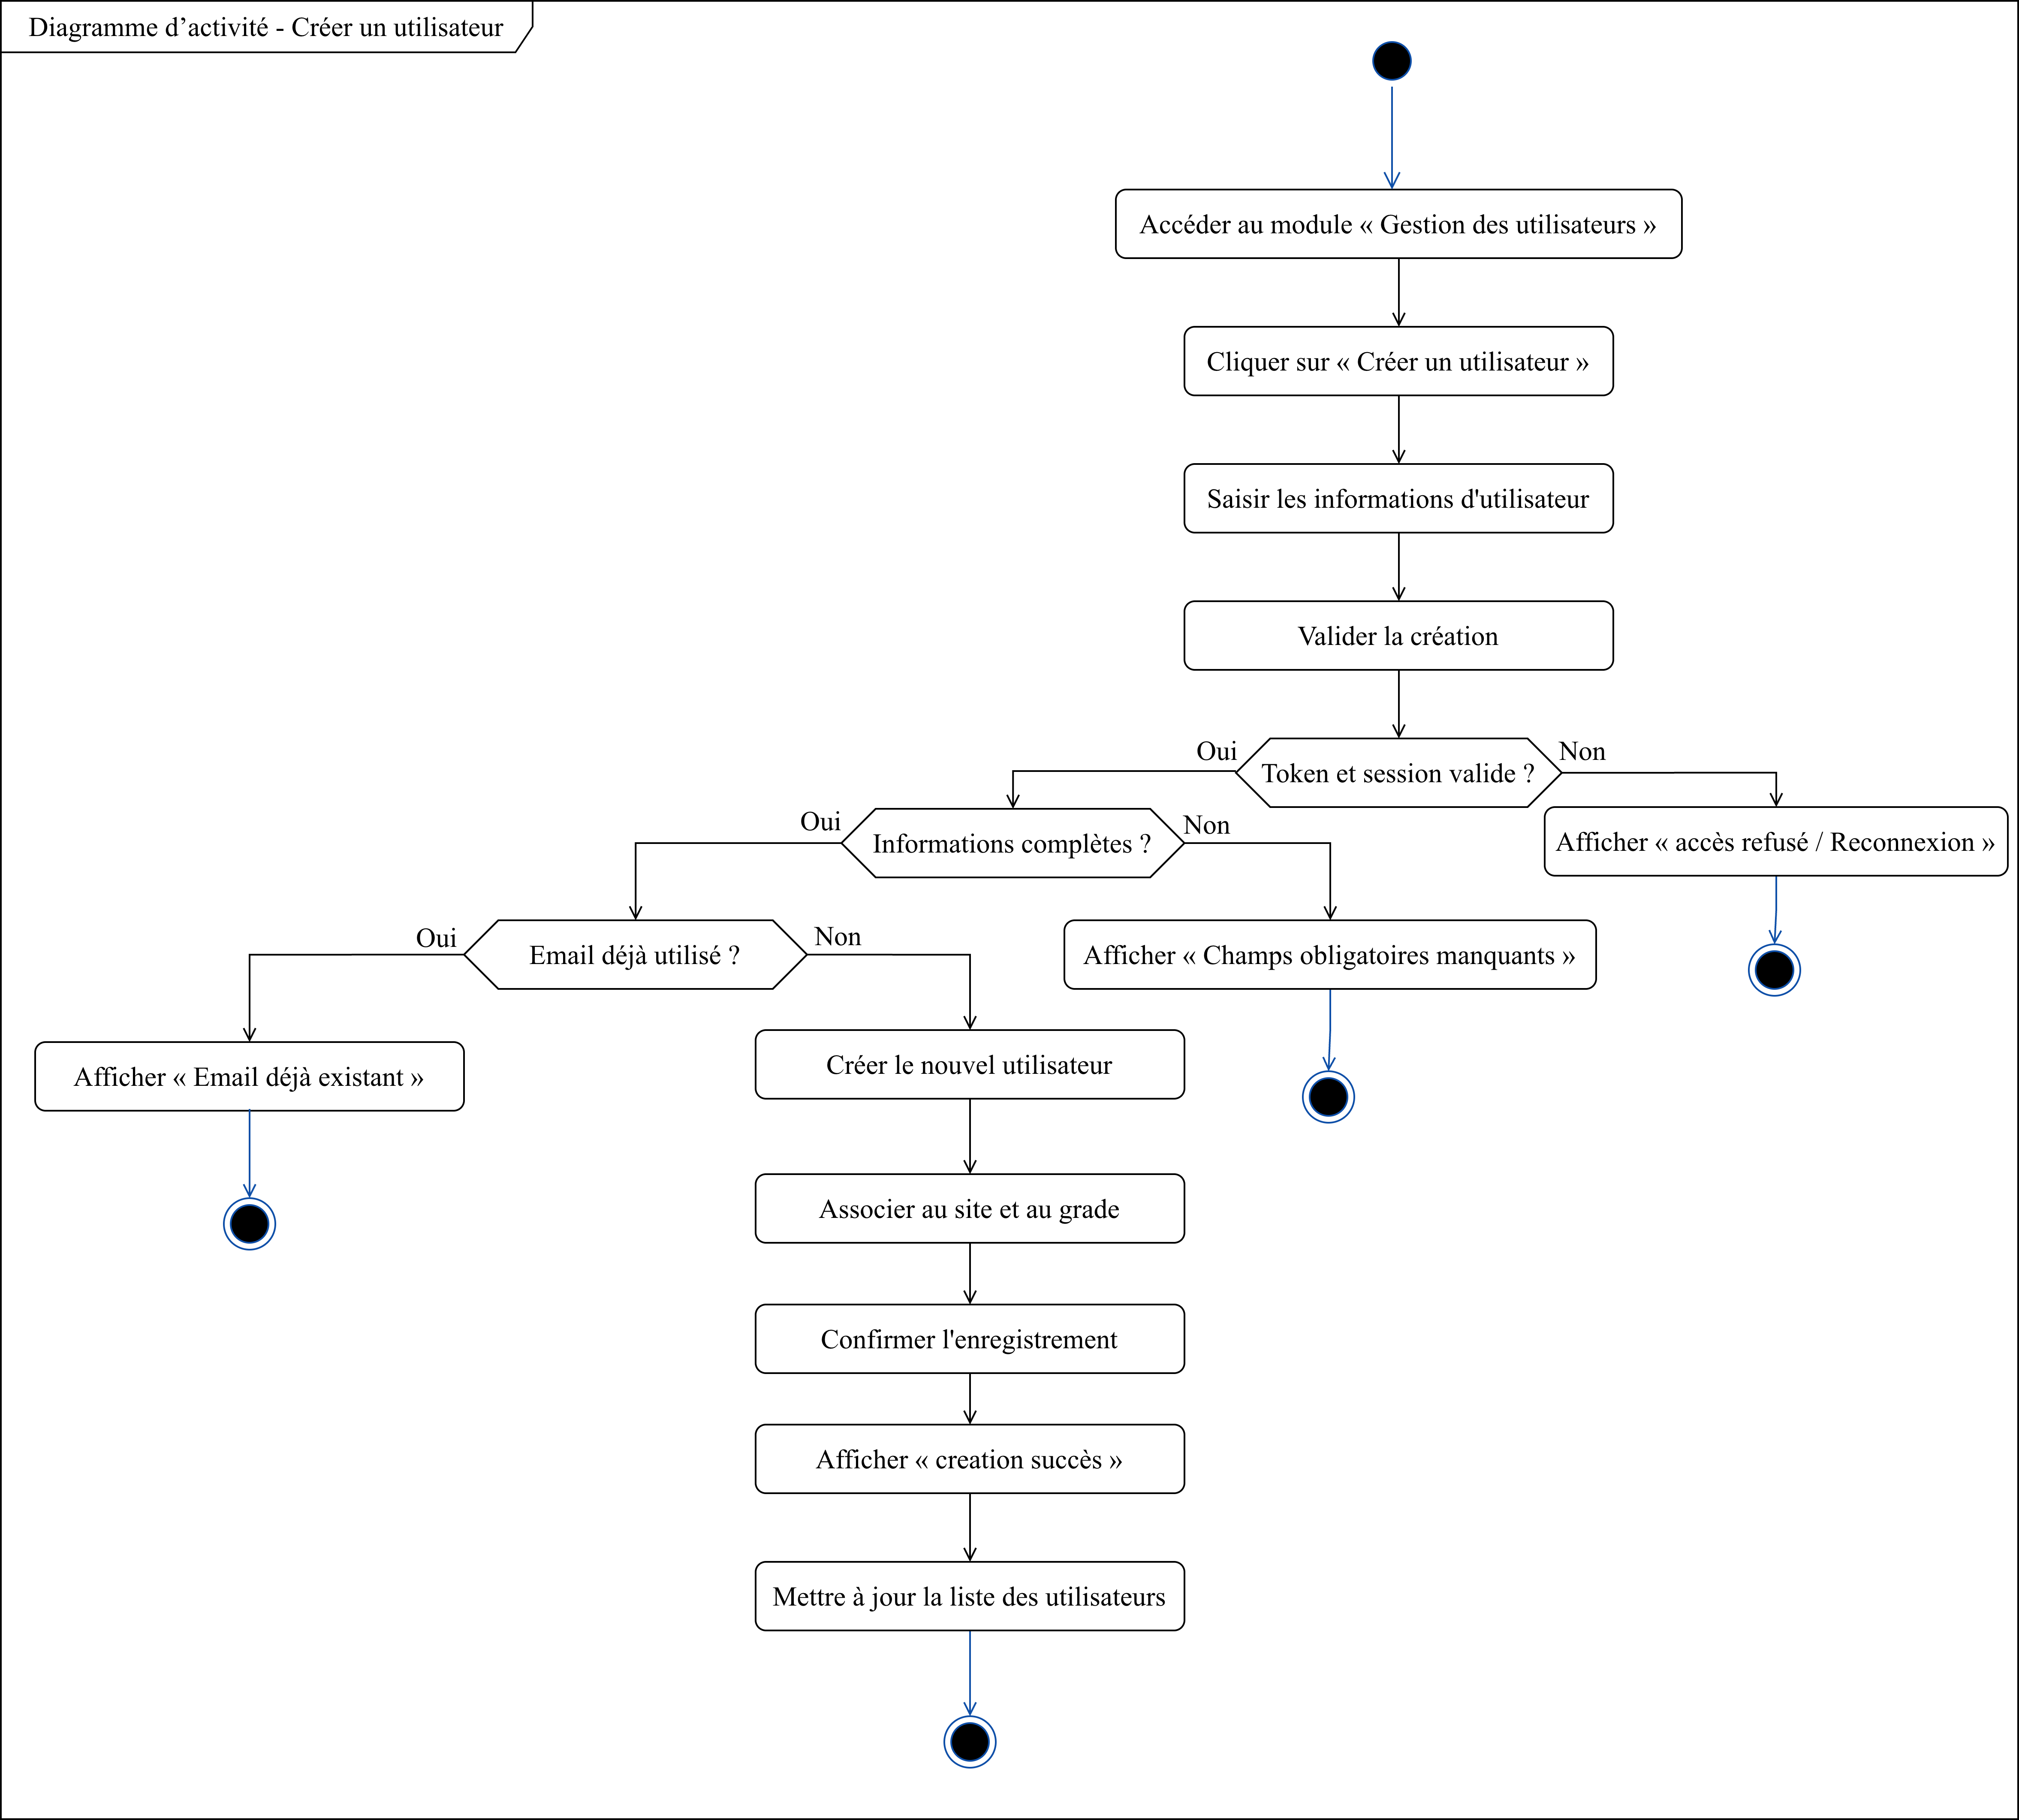
\includegraphics[width=0.92\linewidth]{figures/chapitre-03/Diagramme_dactivite_cree_un_utilisateur.png}
  \caption{Diagramme d’activité — «~Créer un utilisateur~».}
  \label{fig:doc-ch3-act-user}
\end{figure}%
}{%
\begin{figure}[H]
  \centering
  \fbox{\parbox{0.92\linewidth}{\centering\vspace{3.2cm}\textit{(Figure à insérer : \texttt{figures/chapitre-03/Diagramme\_dactivite\_cree\_un\_utilisateur.png})}\vspace{3.2cm}}}
  \caption{Diagramme d’activité — «~Créer un utilisateur~».}
  \label{fig:doc-ch3-act-user}
\end{figure}%
}

\section{Réalisation}

Dans cette section, nous illustrons le travail réalisé durant ce sprint à travers un ensemble de captures d’écran de la plateforme. Ces visuels permettent de mettre en évidence les principales fonctionnalités développées et d'avoir une vision concrète du résultat obtenu.

La figure~\ref{fig:doc-ch3-3} présente l’interface de la liste des utilisateurs.

\begin{figure}[H]
  \centering
  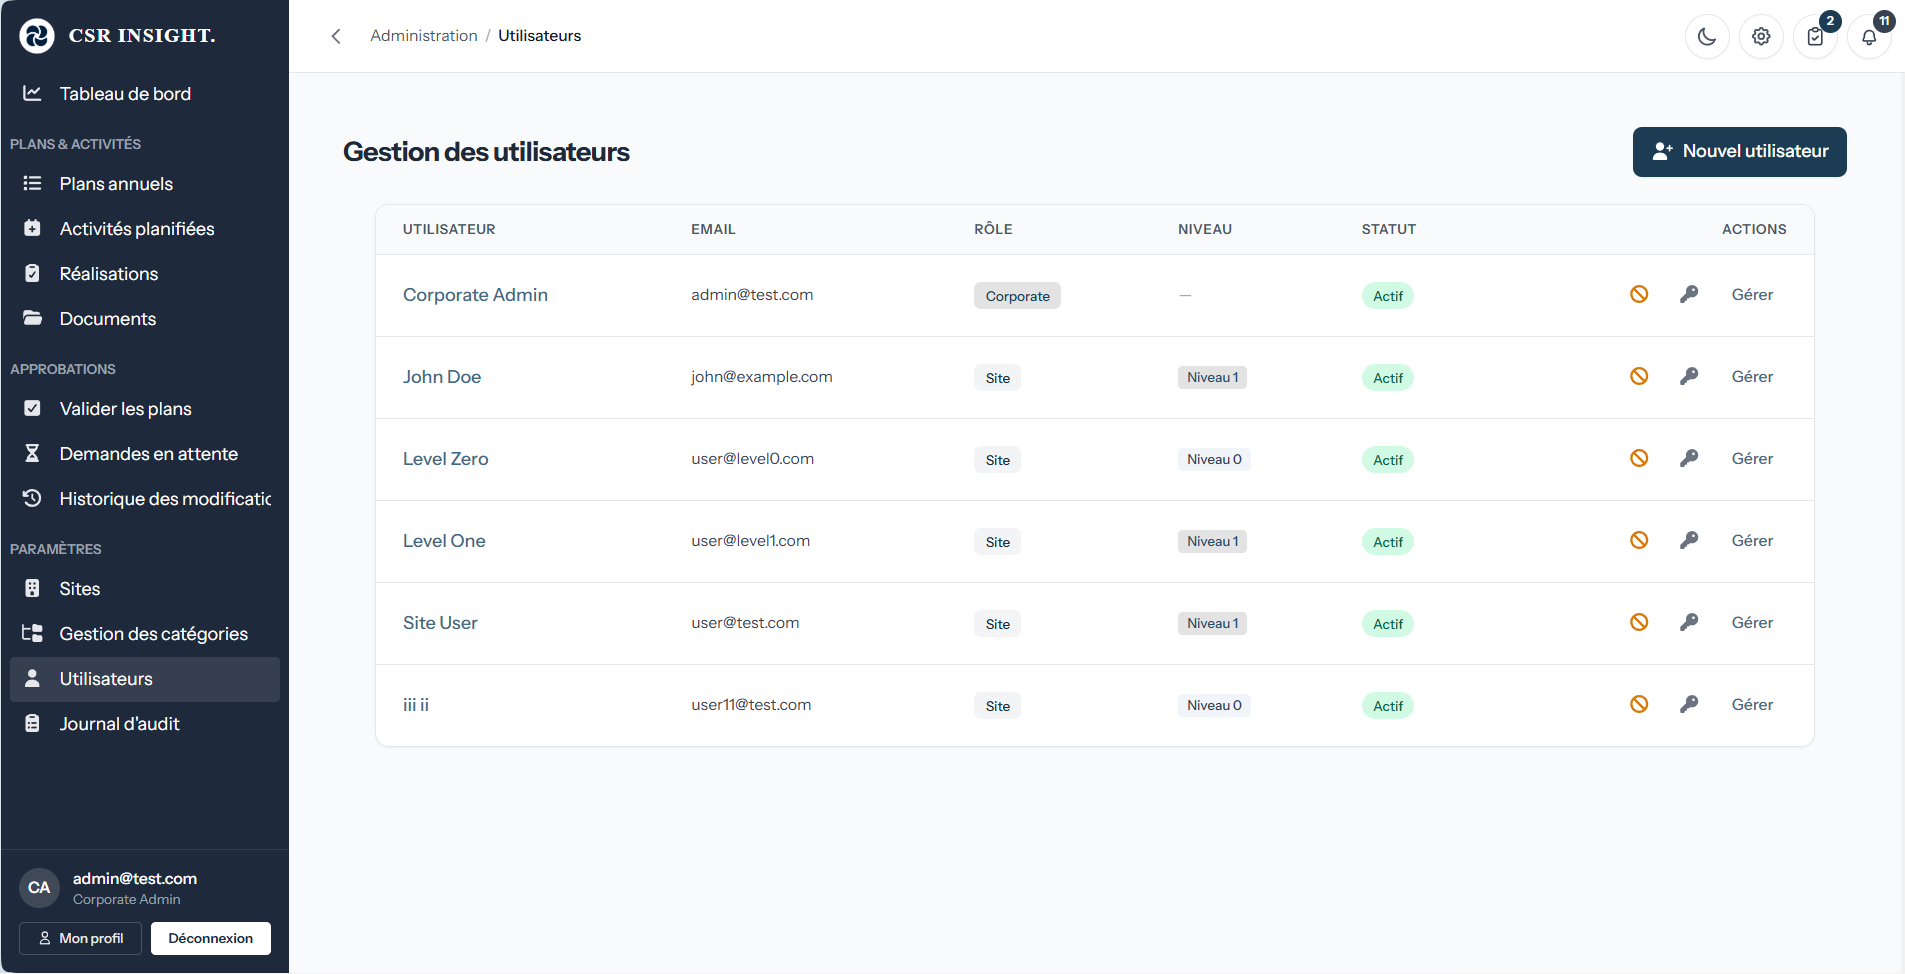
\includegraphics[width=0.92\linewidth]{figures/chapitre-03/ui-gestion-utilisateurs.png}
  \caption{Interface - gestion des utilisateurs.}
  \label{fig:doc-ch3-3}
\end{figure}

Cette interface présente la page de gestion des utilisateurs de la plateforme. Elle permet à l’utilisateur Corporate de consulter les comptes enregistrés via un tableau affichant le nom, le rôle, le niveau d’approbation et le statut. Elle offre également des fonctionnalités de gestion telles que l’ajout, la modification et la désactivation des utilisateurs.

La figure~\ref{fig:doc-ch3-4} présente l’interface de la liste des sites.
\newpage
\begin{figure}[H]
  \centering
  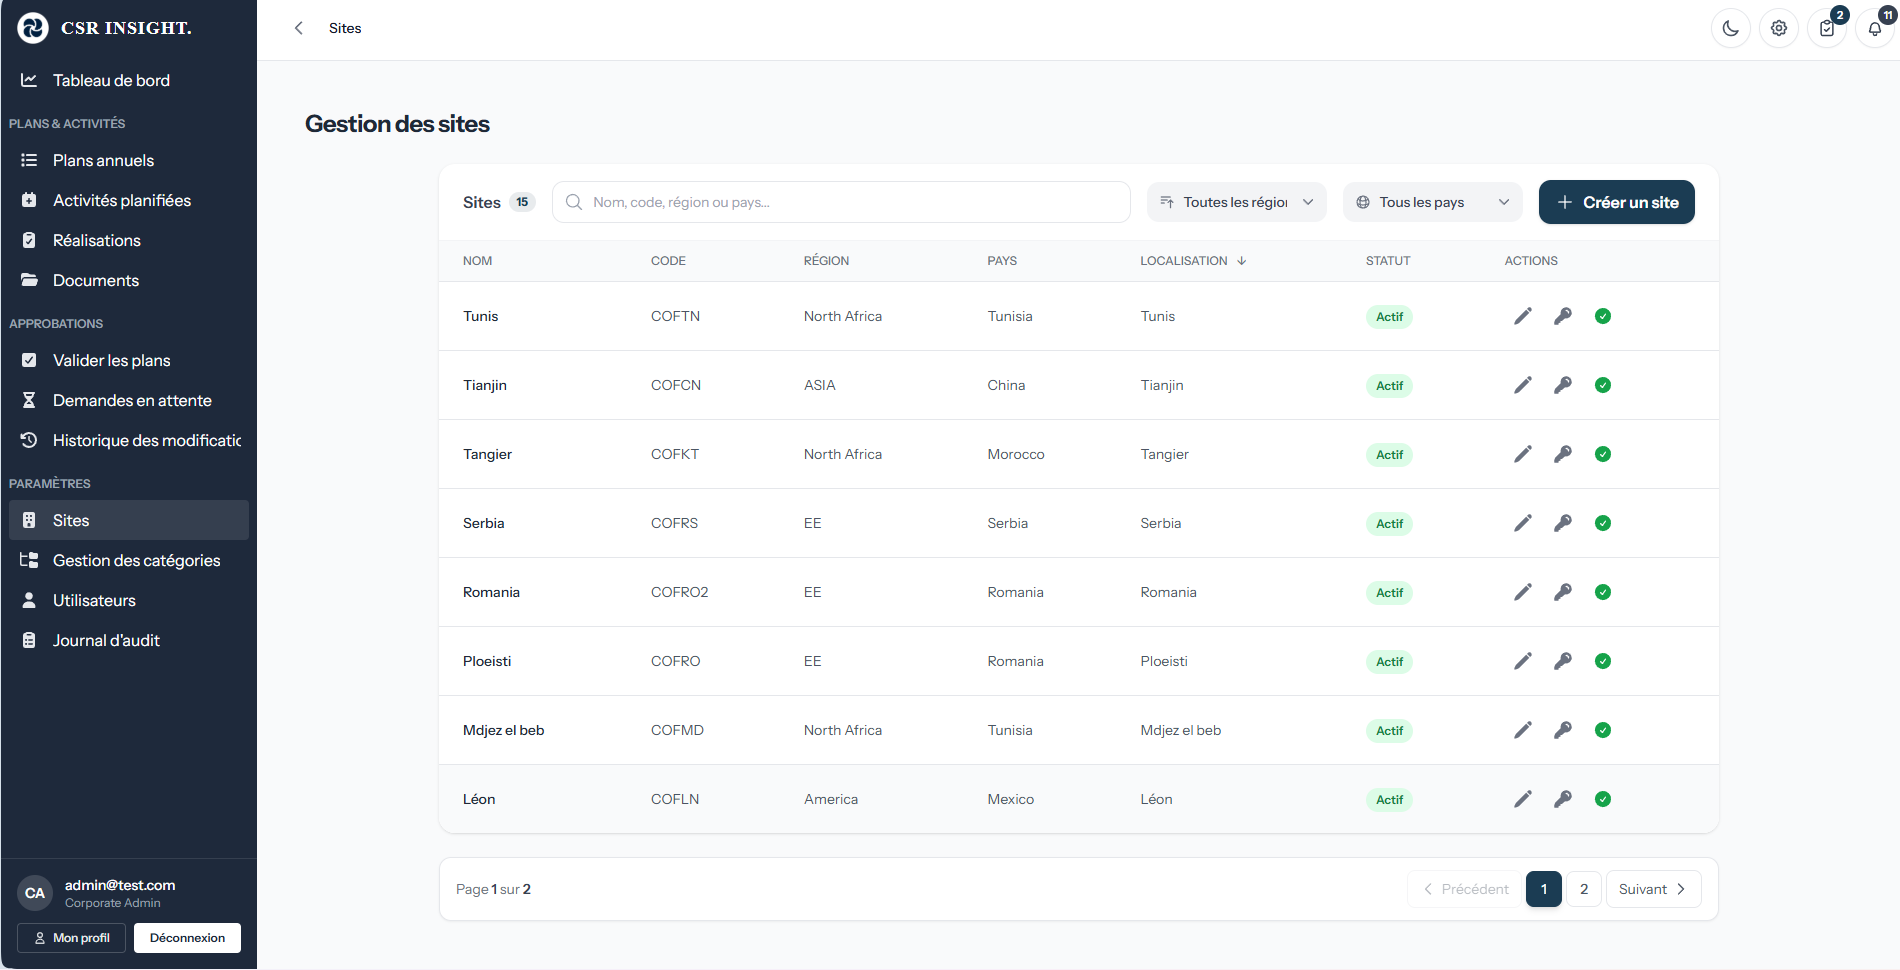
\includegraphics[width=0.92\linewidth]{figures/chapitre-03/ui-gestion-sites.png}
  \caption{Interface - gestion des sites.}
  \label{fig:doc-ch3-4}
\end{figure}

Cette interface présente la page Gestion des sites de la plateforme, dédiée à l’administration et à la configuration des différents sites opérationnels de Coficab à l’échelle internationale. Elle offre une vue centralisée sous forme de tableau listant les sites avec leurs informations essentielles, notamment le nom, le code, la région, le pays, ainsi que leur localisation géographique et leur statut d’activation.

La page intègre des fonctionnalités avancées de recherche et de filtrage permettant d’affiner l’affichage des sites selon plusieurs critères tels que la région ou le pays, facilitant ainsi l’analyse et la gestion dans un contexte multi-sites. L’utilisateur Corporate peut également créer un nouveau site via un bouton dédié, ou effectuer des actions spécifiques sur chaque entrée (modification, activation ou ajouter des utilisateurs à un site bien précis ).


La figure~\ref{fig:doc-ch3-6} présente l’interface de gestion des documents.

\IfFileExists{figures/chapitre-03/ui-gestion-documents.png}{%
\begin{figure}[H]
  \centering
  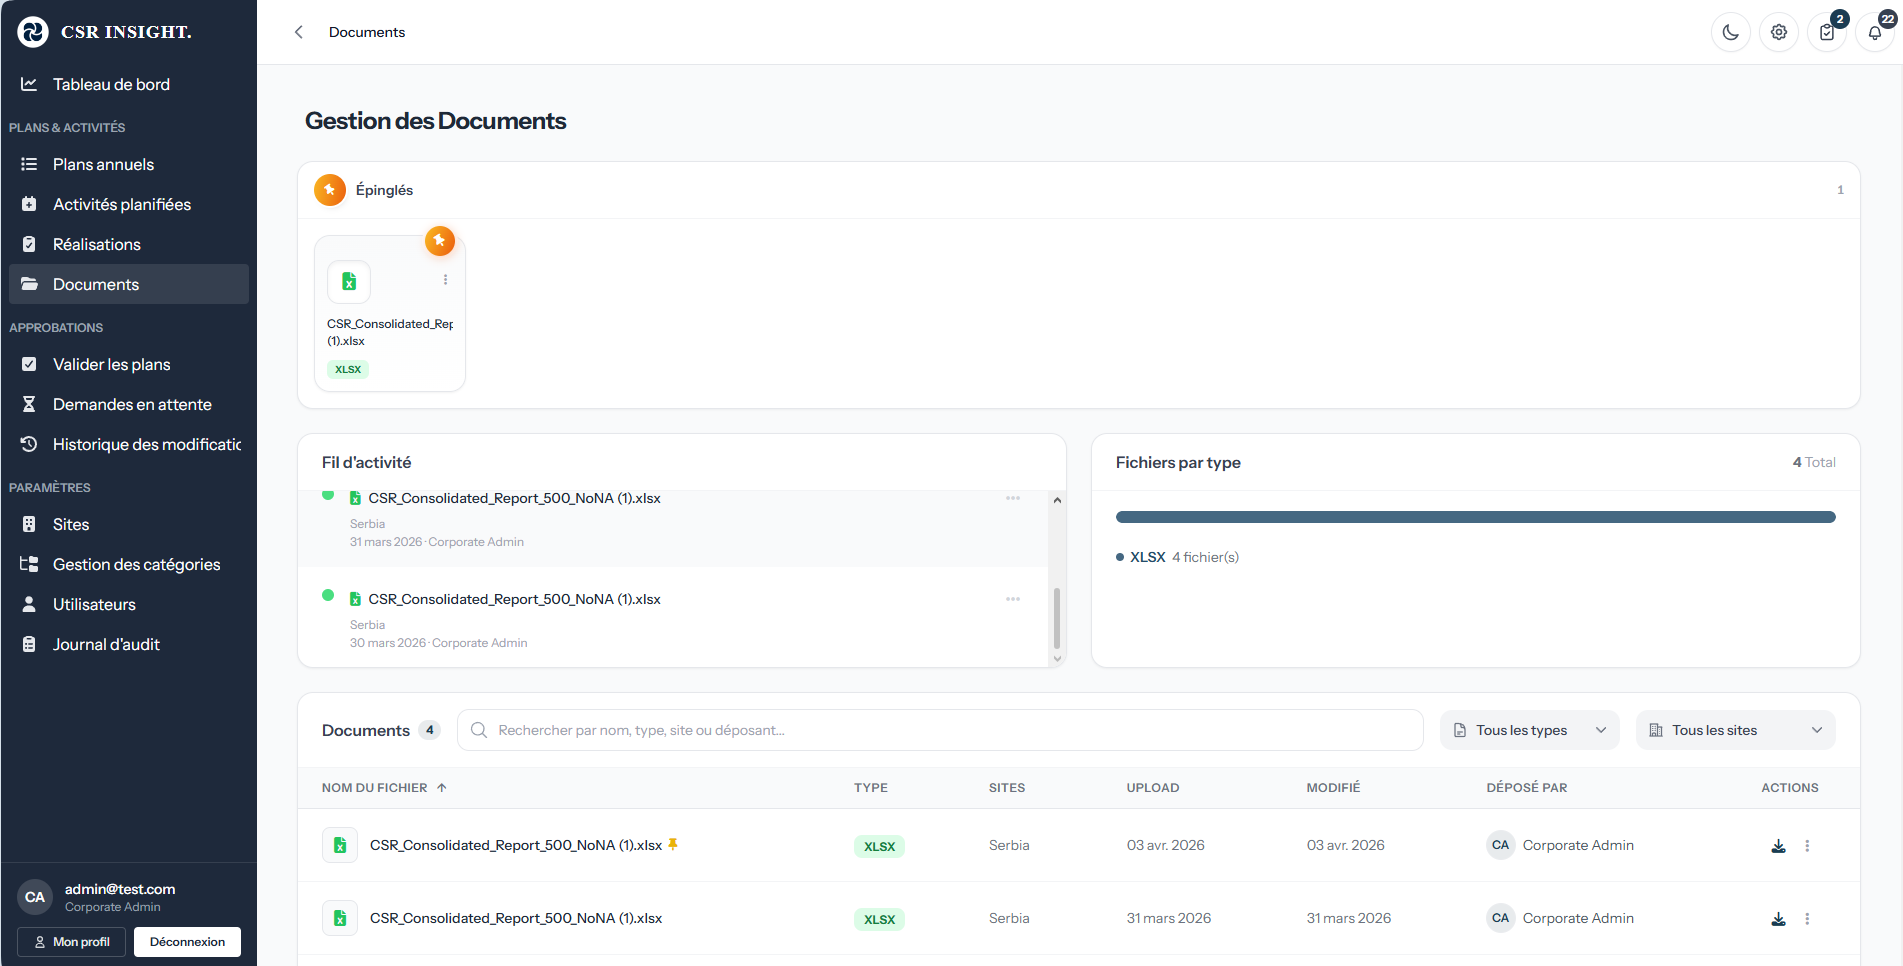
\includegraphics[width=0.92\linewidth]{figures/chapitre-03/ui-gestion-documents.png}
  \caption{Interface : gestion des documents.}
  \label{fig:doc-ch3-6}
\end{figure}%
}{%
\begin{figure}[H]
  \centering
  \fbox{\parbox{0.92\linewidth}{\centering\vspace{3.2cm}\textit{(Figure à insérer : \texttt{figures/chapitre-03/ui-gestion-documents.png})}\vspace{3.2cm}}}
  \caption{Interface : gestion des documents.}
  \label{fig:doc-ch3-6}
\end{figure}%
}

\section{Tests et validation}

Les tests jouent un rôle essentiel dans la méthodologie agile~: ils contribuent à la qualité et à la fiabilité des fonctionnalités livrées. Avant d’enclencher un nouveau sprint, il est nécessaire de vérifier les incréments prioritaires afin de s’assurer du bon fonctionnement et de l’adéquation avec les besoins des acteurs.

\subsection{Test}

Dans cette partie, nous présentons une validation fonctionnelle synthétique des principales fonctionnalités du premier sprint «~Authentification \& Architecture de base~», en couvrant l'\textbf{authentification}, la \textbf{gestion des utilisateurs} et la \textbf{gestion des sites} à travers un tableau consolidé de cas de test.




Le tableau~\ref{tab:ch3-scenarios-tests} présente une synthèse consolidée des cas de test du sprint 1.
% Scénarios de test consolidés — chapitre 3 (authentification, utilisateurs, sites)
\small
\PFETableSetup
\setlength{\LTpre}{0pt}
\setlength{\LTpost}{0pt}
\setlength{\LTleft}{-0.8cm}
\setlength{\LTright}{-0.8cm}
\renewcommand{\arraystretch}{1.25}

\begin{longtable}{|>{\centering\arraybackslash}m{3.1cm}|
>{\raggedright\arraybackslash}p{2.9cm}|
>{\raggedright\arraybackslash}p{4.4cm}|
>{\raggedright\arraybackslash}p{5.0cm}|
>{\centering\arraybackslash}p{1.3cm}|}
\caption{Synthèse des cas de test — Authentification \& Architecture de base}\label{tab:ch3-scenarios-tests}\\
\hline
\tableHeaderStyle
\tableHeaderCell{Nom du cas d'utilisation} &
\tableHeaderCell{Cas de test} &
\tableHeaderCell{Description du cas} &
\tableHeaderCell{Résultat attendu} &
\tableHeaderCell{Résultat réel} \\
\hline
\endfirsthead
\hline
\multicolumn{5}{|c|}{\tablename\ \thetable{} --- \textit{(suite)}} \\
\hline
\tableHeaderStyle
\tableHeaderCell{Nom du cas d'utilisation} &
\tableHeaderCell{Cas de test} &
\tableHeaderCell{Description du cas} &
\tableHeaderCell{Résultat attendu} &
\tableHeaderCell{Résultat réel} \\
\hline
\endhead
\hline
\multicolumn{5}{|r|}{\textit{Suite page suivante\ldots}} \\
\hline
\endfoot
\hline
\endlastfoot

\multirow{2}{=}{\centering S'authentifier} &
Identifiants manquants &
Tentative de connexion sans renseigner l'email ou le mot de passe. &
Message indiquant que les champs d'authentification sont obligatoires. &
Vrai \\
\cline{2-5}

 &
Identifiants invalides &
Tentative de connexion avec des informations incorrectes. &
Message d'échec d'authentification. &
Vrai \\
\hline

Accéder à Dashboard &
Utilisateur non authentifié &
L'utilisateur tente d'accéder au tableau de bord sans session valide. &
Redirection vers la page de connexion ou message d'accès refusé. &
Vrai \\
\hline

\multirow{5}{=}{\centering Gérer \\les utilisateurs} &
Afficher la liste des utilisateurs &
Ouverture du module de gestion des utilisateurs par un profil autorisé. &
La liste des utilisateurs s'affiche correctement. &
Vrai \\
\cline{2-5}

 &
Créer un utilisateur &
Création d'un nouveau compte avec des informations valides. &
Le compte est créé et apparaît dans la liste. &
Vrai \\
\cline{2-5}

 &
Modifier un utilisateur &
Mise à jour des informations d'un utilisateur existant. &
Les modifications sont enregistrées et visibles. &
Vrai \\
\cline{2-5}

 &
Désactiver un utilisateur &
Changement du statut d'un utilisateur actif vers inactif. &
Le compte est désactivé et l'état est mis à jour dans la liste. &
Vrai \\
\cline{2-5}

 &
Associer un utilisateur à un site avec un grade &
Attribution d'un utilisateur à un site avec un niveau de grade. &
L'affectation et le grade sont enregistrés correctement. &
Vrai \\
\hline

\multirow{4}{=}{\centering Gérer les sites} &
Créer un site &
Création d'un site avec les informations requises. &
Le site est créé et visible dans la liste des sites. &
Vrai \\
\cline{2-5}

 &
Modifier un site &
Modification des informations d'un site existant. &
Les nouvelles informations du site sont enregistrées. &
Vrai \\
\cline{2-5}

 &
Désactiver un site &
Passage d'un site actif en état désactivé. &
Le site est désactivé et n'est plus proposé aux actions actives. &
Vrai \\
\cline{2-5}

 &
Consulter un site &
Consultation des détails d'un site depuis la liste. &
Les informations détaillées du site sont affichées. &
Vrai \\
\hline

\multirow{4}{=}{\centering Gérer \\les documents} &
Télécharger un fichier &
Ajout d'un document dans la plateforme. &
Le fichier est importé et disponible dans la liste des documents. &
Vrai \\
\cline{2-5}

 &
Modifier un fichier &
Mise à jour des informations ou métadonnées d'un document existant. &
Les modifications sont enregistrées et visibles. &
Vrai \\
\cline{2-5}

 &
Supprimer un fichier &
Suppression d'un document depuis la gestion documentaire. &
Le fichier est supprimé et n'apparaît plus dans la liste. &
Vrai \\
\cline{2-5}

 &
Gérer les documents &
Accès global aux actions de consultation et de gestion documentaire. &
Les actions autorisées sont accessibles selon le profil utilisateur. &
Vrai \\
\hline

\end{longtable}
\normalsize

\subsubsection{Tests authentification}

Les captures Postman illustrent le contrôle du point d’accès \textbf{/api/auth/login} dans deux scénarios complémentaires. 
\begin{itemize}
\item Dans le premier cas (succès), la soumission de credentials valides retourne le statut \textbf{200 OK} ainsi que les informations de l’utilisateur connecté et un \textbf{token} d’authentification, validant le bon fonctionnement du mécanisme de connexion et de sécurisation de la session.
\item Dans le second cas (échec), l’envoi d’un mot de passe incorrect pour un email existant retourne le statut \textbf{401 Unauthorized} avec un message explicite («~Email ou mot de passe incorrect.~»), ce qui confirme le rejet des identifiants invalides. 
\end{itemize}
Les figures~\ref{fig:ch3-postman-auth-success} et~\ref{fig:ch3-postman-auth-failure} présentent les cas succès/échec pour l'authentification.

\begin{figure}[H]
  \centering
  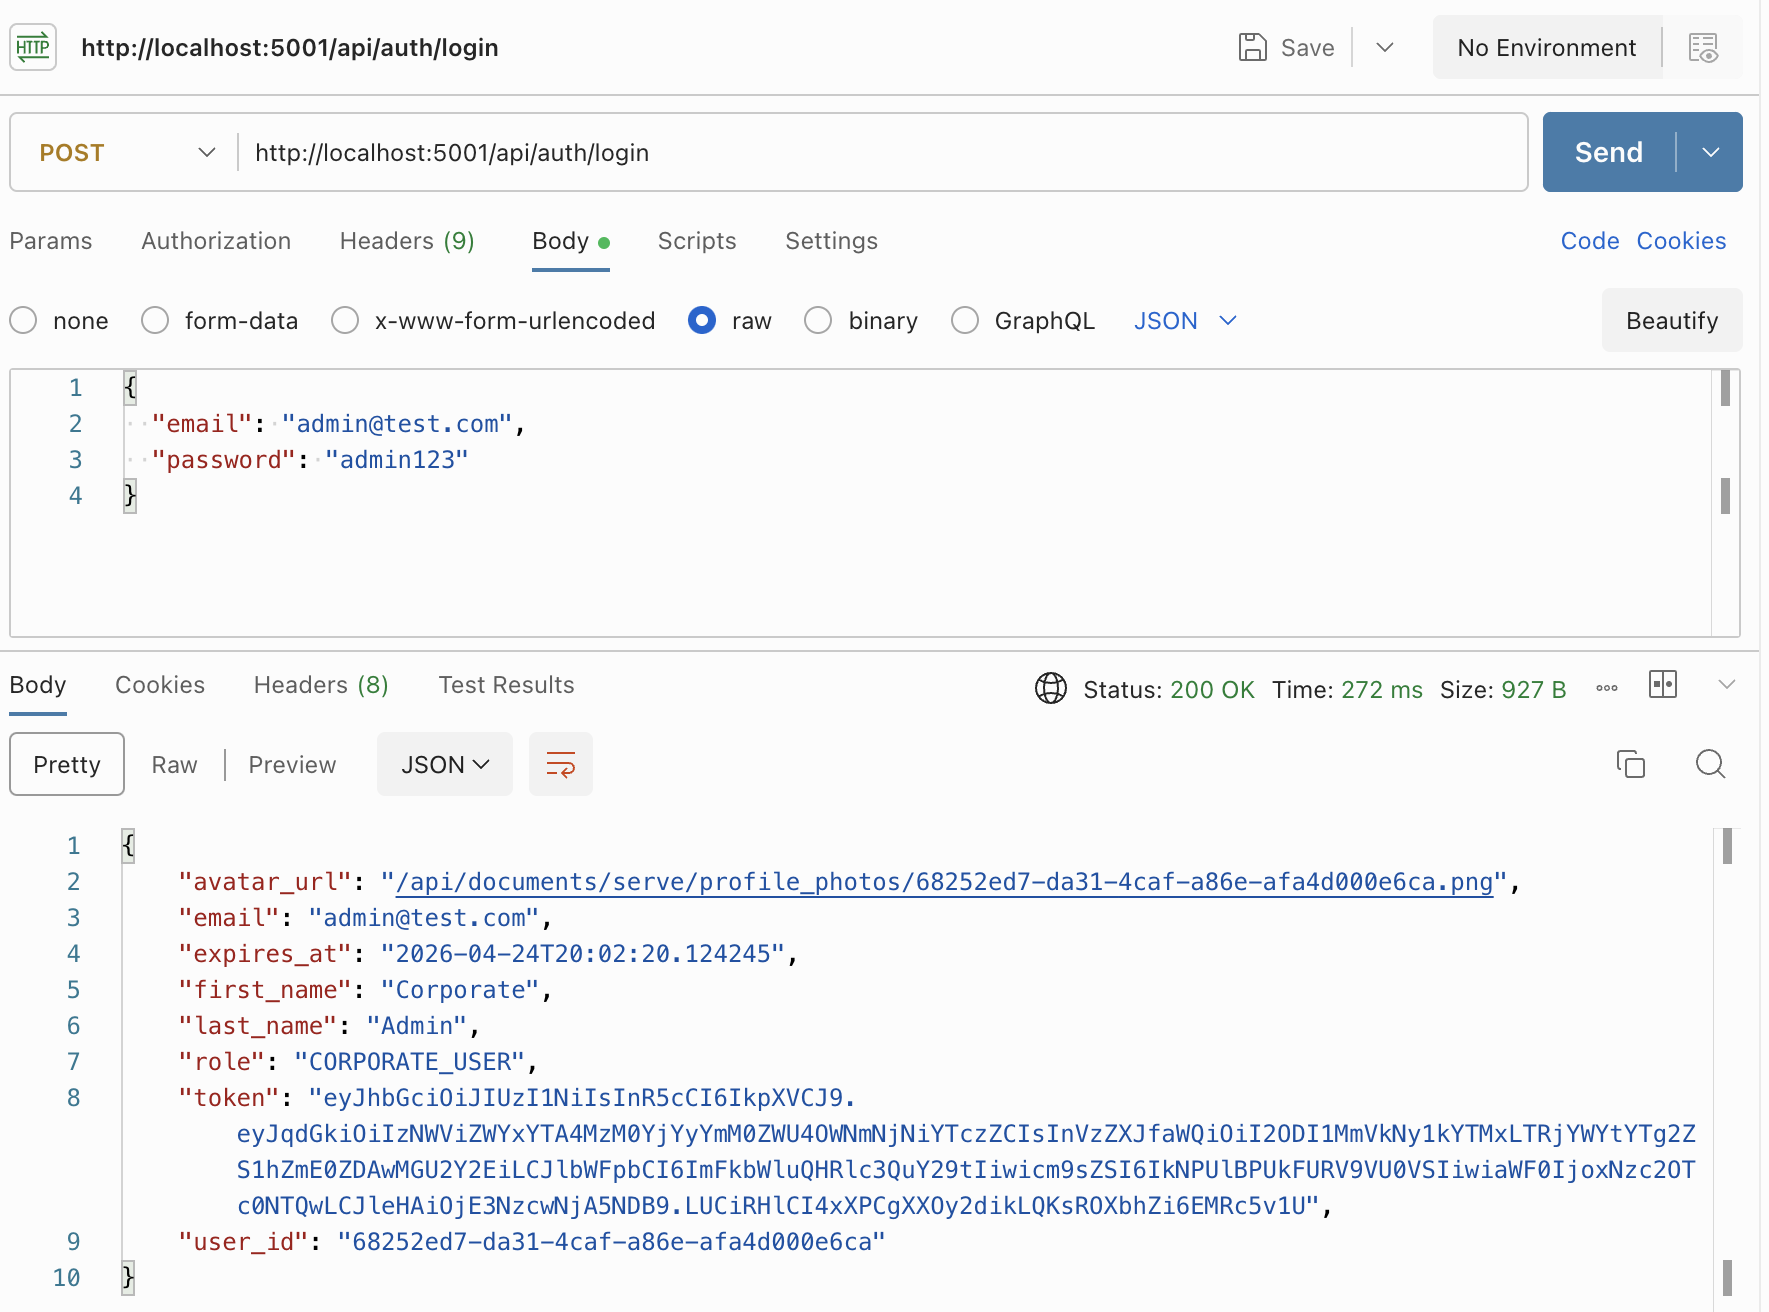
\includegraphics[width=1\linewidth]{figures/chapitre-03/postman-auth-success.png}
  \caption{Tests Postman : authentification réussie.}
  \label{fig:ch3-postman-auth-success}
\end{figure}                 

\begin{figure}[H]
  \centering
  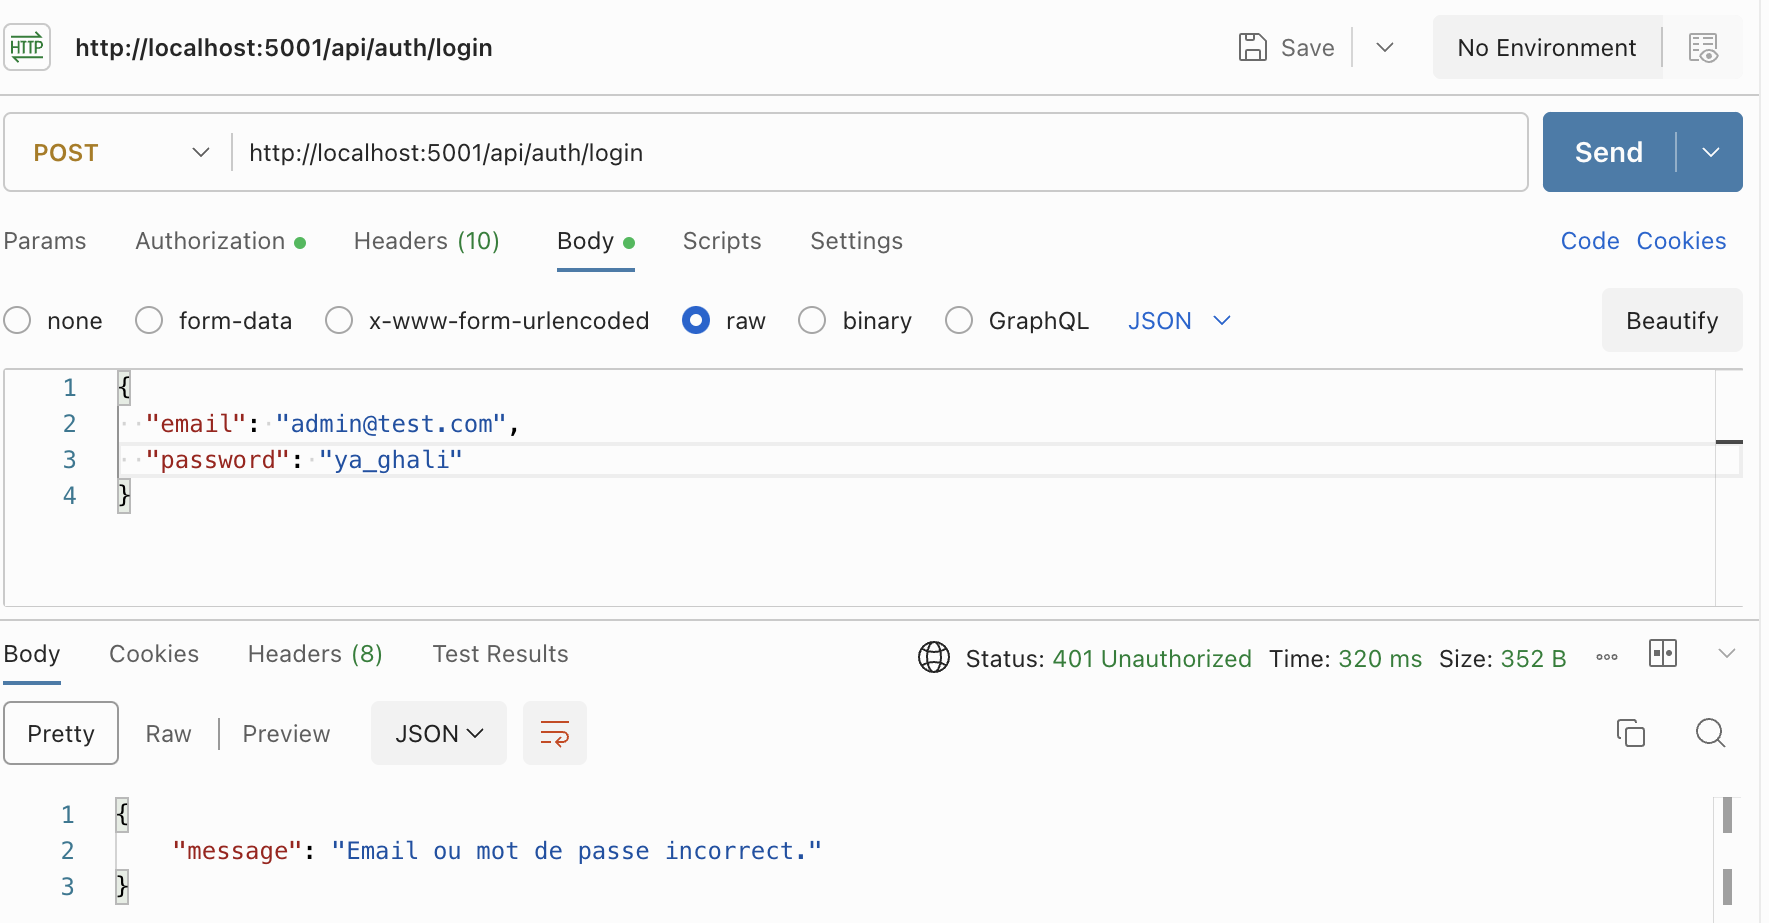
\includegraphics[width=1\linewidth]{figures/chapitre-03/postman-auth-failure.png}
  \caption{Tests Postman : authentification échouée.}
  \label{fig:ch3-postman-auth-failure}
\end{figure}
\subsubsection{Tests création d'un utilisateur}

Les figures~\ref{fig:ch3-postman-user-create-success} et~\ref{fig:ch3-postman-user-create-failure} présentent les cas succès/échec pour la création d'un utilisateur.

Les captures Postman illustrent la vérification du point d’accès \textbf{/api/users} dans deux scénarios complémentaires.
\begin{itemize}
\item Dans le premier cas (succès), l’envoi d’un payload valide pour un nouvel utilisateur retourne le statut \textbf{201 Created} avec les informations du compte créé (identifiant, email, nom, rôle et date de création), ce qui confirme la bonne exécution du processus d’ajout.
\item Dans le second cas (échec), la tentative de création avec un email déjà existant retourne le statut \textbf{409 Conflict} accompagné du message «~Un utilisateur avec cet email existe déjà~», validant le contrôle d’unicité appliqué par l’API.
\end{itemize}

\begin{figure}[H]
  \centering
  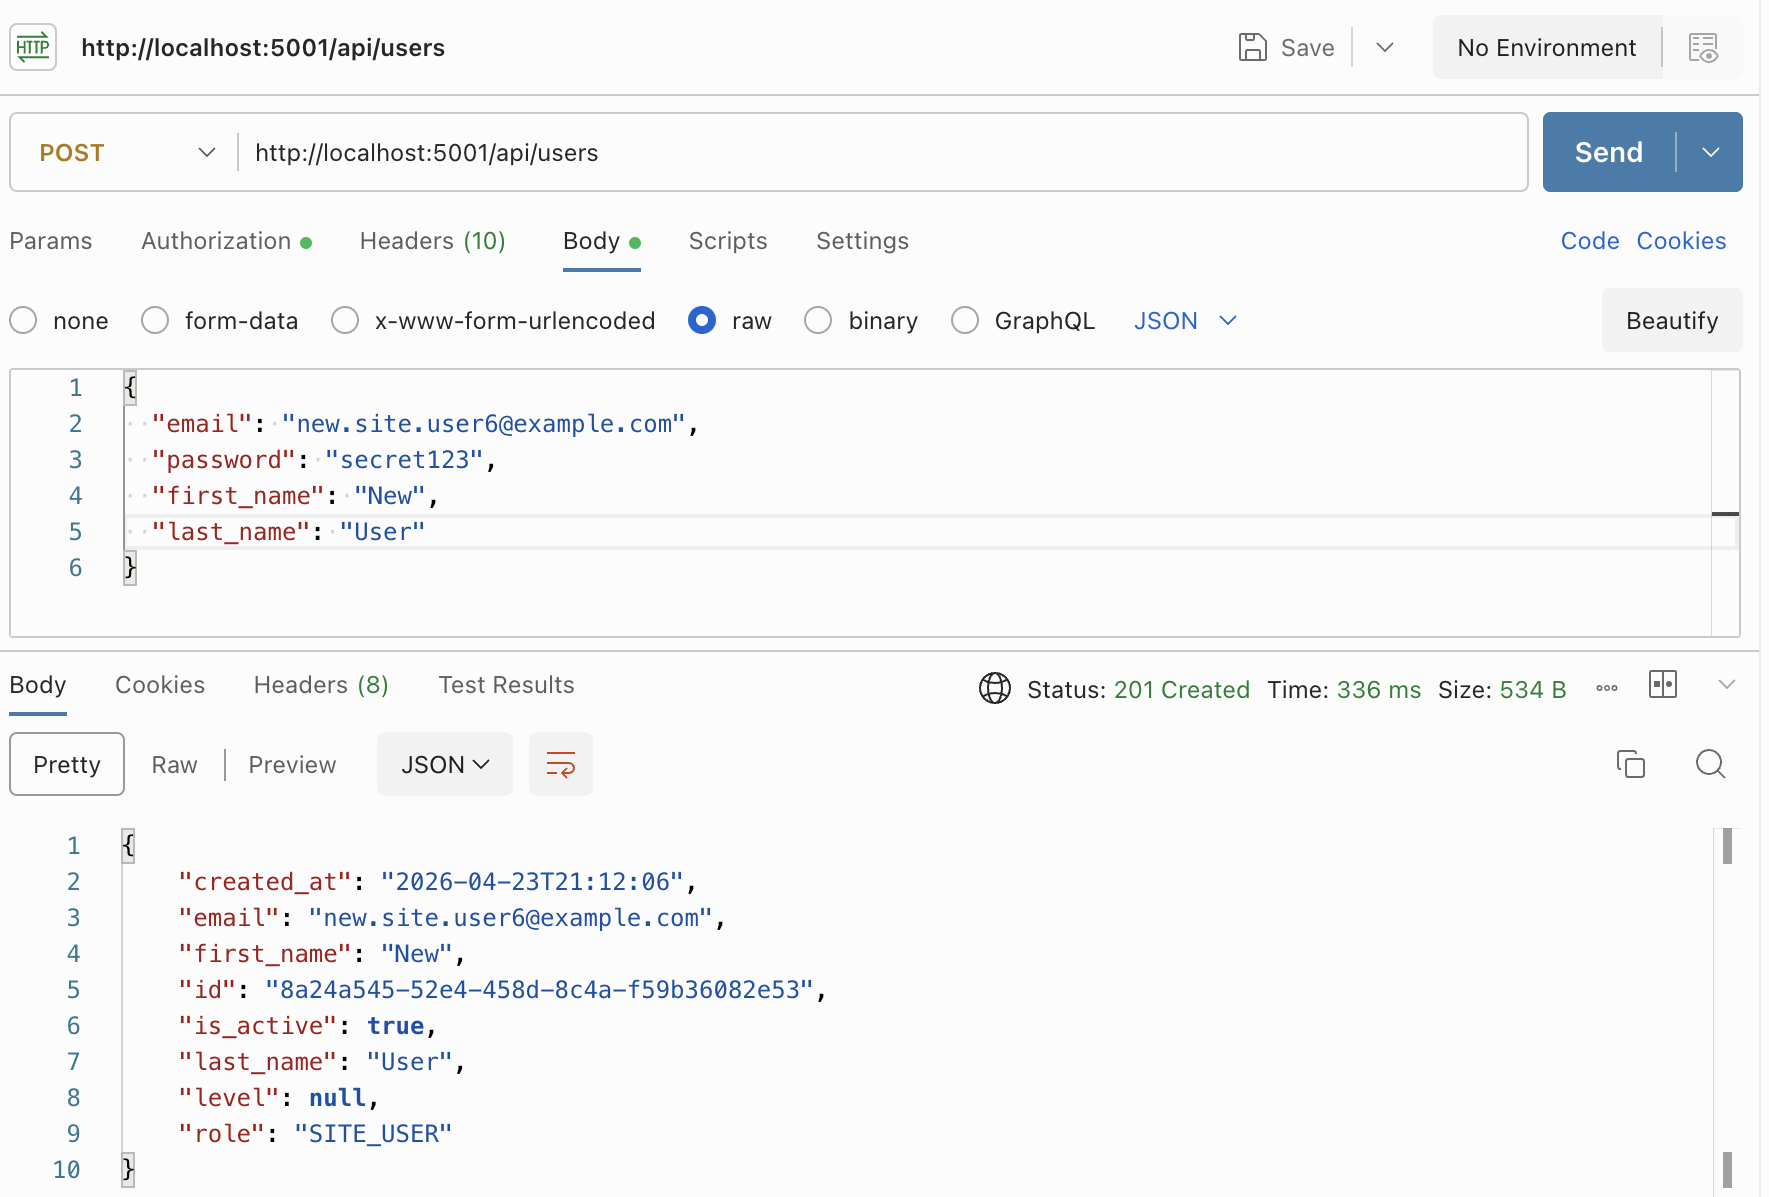
\includegraphics[width=1\linewidth]{figures/chapitre-03/postman-user-create-success.png}
  \caption{Tests Postman : création d'un utilisateur réussie.}
  \label{fig:ch3-postman-user-create-success}
\end{figure}

\begin{figure}[H]
  \centering
  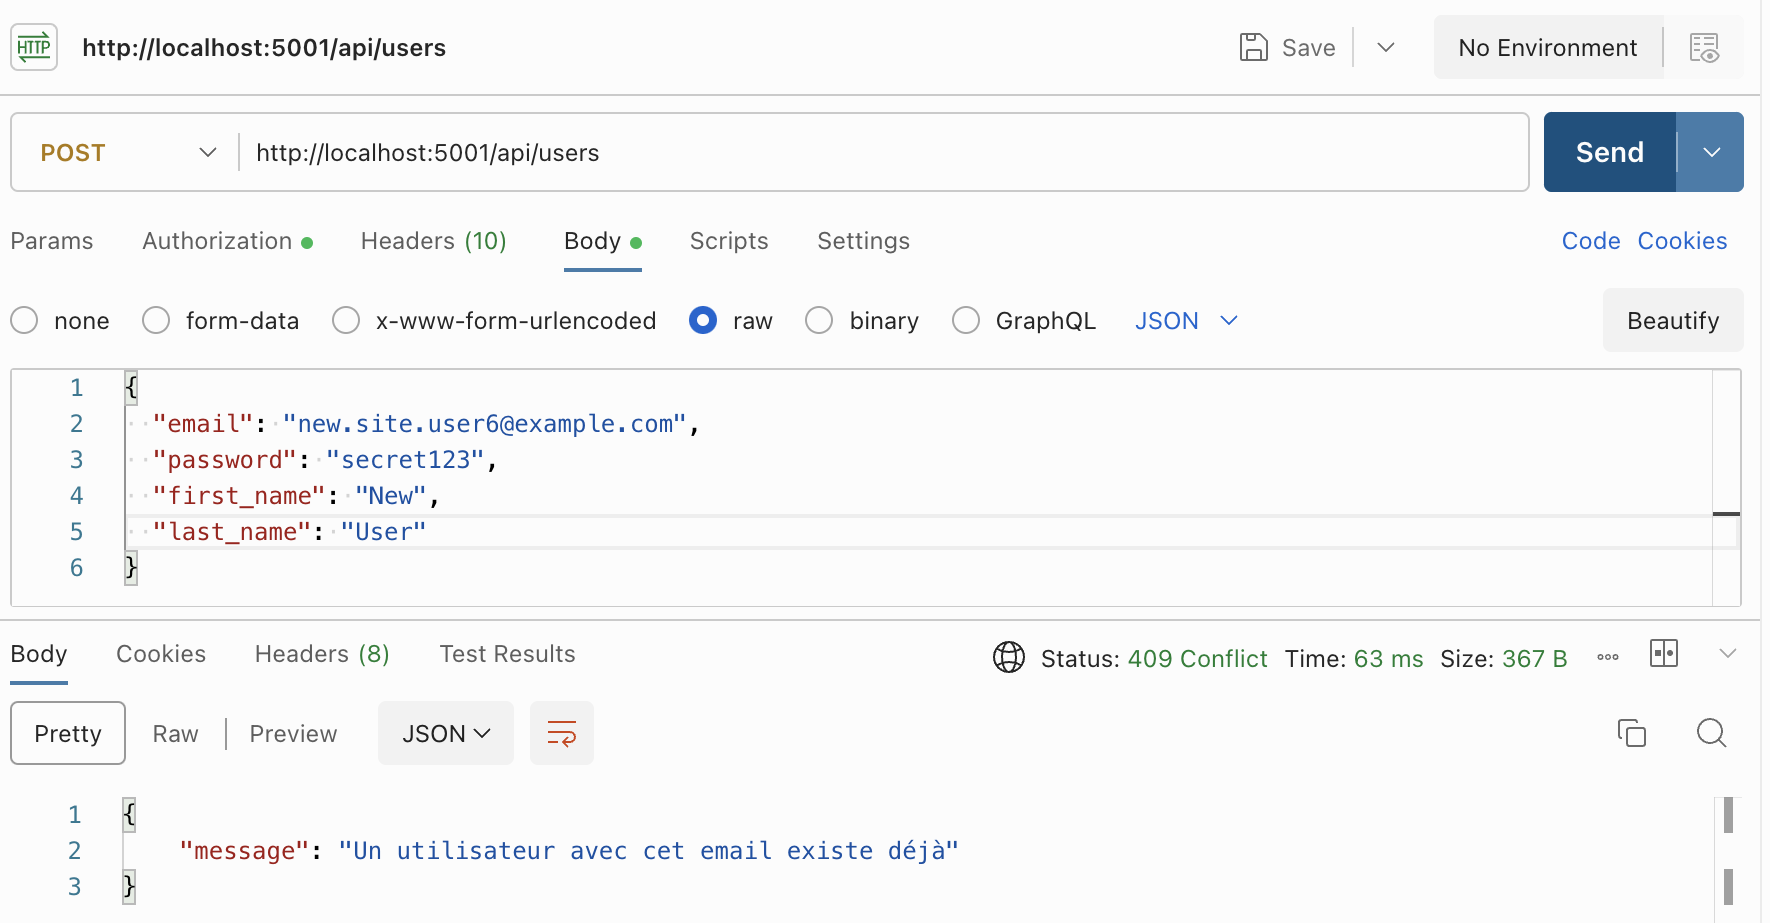
\includegraphics[width=1\linewidth]{figures/chapitre-03/postman-user-create-failure.png}
  \caption{Tests Postman : création d'un utilisateur échouée.}
  \label{fig:ch3-postman-user-create-failure}
\end{figure}


\subsection{Validation}

À la fin du sprint, une réunion de revue a été animée par le \emph{Scrum Master} et le \emph{Product Owner}. Elle a permis de tester les fonctionnalités livrées sur la plateforme CSR (authentification, gestion des utilisateurs, gestion des sites) et de valider leur bon fonctionnement sur les scénarios prioritaires.

Les tests effectués ont confirmé la fiabilité des parcours de gestion des utilisateurs et des sites dans le périmètre de ce sprint. Les éventuels écarts d’affichage ou de formulation signalés lors de la démonstration ont été corrigés afin d’offrir une expérience utilisateur plus claire pour la suite du projet.

\section{Conclusion}

Ce premier sprint a permis de mettre en place les bases essentielles de la plateforme : gestion des utilisateurs, des sites, des accès et des documents. Les fonctionnalités ont été développées et validées, constituant un socle fiable pour la suite du projet.
